\chapter[Eigene "Uberlegungen und die Implementierung]{Eigene "Uberlegungen und die Implementierung der resultierenden L"osung}
\minitoc
\newpage
\section{Vor"uberlegungen} \label{vorueberlegungen}
Im Folgenden werden die Vorschl"age aus der Literatur, die oben beschrieben worden sind, bewertet und einige Gedanken ausgeführt, die zum Thema Matching gemacht wurden. Außerdem wird  angegeben, welche dieser Vorschläge verwirklicht wurden und welche noch auf ihre Implementierung warten.

\subsection[Bewertung der Vorschl"age aus \cite{TG}]{Bewertung der Vorschl"age aus ,,Creating Representations for Continuously Moving Regions from Observations''\cite{TG}}

Zu den Matchingverfahren, die die Autoren in \cite{TG} vorgestellt haben, wurden folgende Überlegungen angestellt:

\begin{enumerate}
\item Position of centroid\index{Match!Schwerpunkt}

In dem Paper wurde die M"oglichkeit des Matchens mit dem Schwerpunkt nicht weiter betrachtet, da die Autoren davon ausgehen, dass ein Referenzpunkt, der auch au"serhalb des Polygons liegen kann, nicht zu guten Matchings f"uhren kann. Hierzu muss angemerkt werden, dass im Rahmen der vorliegenden Arbeit das Matching auf Ebene des \textit{ConvexHullTrees} durchgef"uhrt wird und lediglich mit konvexen H"ullen von Polygonen gearbeitet wird. Der Schwerpunkt einer konvexen H"ulle liegt aber wieder innerhalb dieser. Wenngleich der Punkt nicht zwangsl"aufig auch innerhalb des repr"asentierten Polygons liegt. Au"serdem erscheint es plausibel, dass ein Referenzpunkt--Verfahren seine St"arke gerade dort haben wird, wo die "Uberlappungsalgorithmen ihre Schw"achen haben, nämlich bei sich relativ schnell bewegenden, kleinen Objekten. Ein Beispiel für solche Objekte wird in Abbildung~\vref{fig:SchnelleBewegung} skizziert.

\begin{figure}
	\centering
	\includegraphics[scale=0.8]{3_1.1.eps}
	\caption[Beispiel für den Vorteil von Referenzpunktverfahren]{Beispiel für viele kleine Flächen, die sich relativ schnell bewegen. Wie man sehen kann, würde ein Überlappungsverfahren hier kein einziges \textit{Match}, das Referenzpunktverfahren aber eventuell alle möglichen finden.\\\textit{Quelle: Eigene Darstellung}}
	\label{fig:SchnelleBewegung}
\end{figure}


Außerdem läßt die Arbeit \cite{AFRW} es sinnvoll erscheinen, diesen Ansatz weiterzuverfolgen.

Der Vorschlag, "`n"achste Nachbarn"' zu benutzen, hat den Nachteil, dass so nur $1$:$1$ Matches gefunden werden. Im Rahmen der vorliegenden Arbeit wurde stattdessen das Schwellwert-Verfahren gew"ahlt. Siehe hierzu \vref{Schwellwert}.

\item Fixend threshold (set of cycles)\index{Match!Überlappung}

Das Verfahren wurde analog zur Beschreibung Erlend T\o{}ssebros, wie in \vref{fixedThre} kurz dargestellt, "ubernommen und implementiert. 

Nach kurzer Überlegung kommt man zu dem Schluss, dass dieses Verfahren Schwächen aufweisen wird, wenn sich kleine Flächen so stark bewegen, dass diese sich nicht mehr, oder nur noch wenig überlappen. Bei kompliziert aufgebauten Flächen, die sich relativ wenig bewegen, wird dieses Verfahren aber den Vorteil aufweisen, dass relativ wenige falsche Flächen gematcht werden. Ein Beispiel für solche Flächen wird in Abbildung~\vref{fig:OverlapVorteil} gezeigt.

\begin{figure}
	\centering
	\includegraphics[scale=0.6]{3.2.eps}
	\caption[Beispiel für den Vorteil des Overlaping-Match]{Beispiel eine \textit{Matches} von komplizierten Regionen. Wie man sehen kann, würde ein Überlappungsmatch nur die richtigen Übereinstimmungen zurückgeben, ein Referenzpunktverfahren aber deutlich mehr.\\\textit{Quelle: Eigene Darstellung}}
	\label{fig:OverlapVorteil}
\end{figure}


\item Maximize Overlap (set of cycles) 

Dieses Verfahren k"onnte interessant sein, da es aber im  Rahmen dieser Arbeit nicht möglich ist, alle interessanten Matchings zu implementieren, wurde auf die Implementierung dieses Matchings verzichtet.

\end{enumerate}

\subsection[Bewertung der Vorschl"age aus \cite{AAR}]{Bewertung der Vorschl"age aus ,,Matching Shapes with a Reference Point'' \cite{AAR}}

Wie unter \vref{BedeutungAAR} bereits ausgeführt wurde, wurde der Algorithmus $S$, der allgemeinste dieser Arbeit, nicht implementiert. Die Idee, ein Match auf Basis des Steiner--Punktes zu implementieren, führte aber dazu, ein Match zu implementieren, das simultan zu dem Verfahren ,,Position of centroid'' aus \cite{TG} funktioniert, aber den SteinerPunkt als Referenzpunkt benutzt.

\subsection[Bewertung der Vorschl"age aus \cite{AFRW}]{Bewertung der Vorschl"age aus ,,Matching Convex Shapes with Respect to Symmetric Difference'' \cite{AFRW}}

Es gilt im Wesentlichen dasselbe wie  im letzten Absatz. Nicht die Algorithmen aus der Arbeit, sondern die beiden Verfahren ,,Fixend threshold'' und ,,Position of centroid'' aus \cite{TG}, wurden implementiert. Wie unter \vref{BedeutungAFRW} ausgeführt wird, weisen beide Verfahren  eine gewisse Verwandtschaft zu dem einfachsten Algorithmus dieser Arbeiten auf. 


\subsection{\index{Match!Referenzpunkt}Matching mit Referenzpunkten}

Die meisten Matching-Verfahren basieren auf Referenzpunkten. Unter \vref{AARR} und \vref{AFRWW} wurden Verfahren angegeben, die zu bestimmten Referenzpunkten Matchings mit garantierter Qualität liefern. Es folgten nun einige Gedanken darüber, wie man Referenzpunktverfahren durchführen könnte.


\subsubsection*{Statistische Analyse}\label{StatistikAlgo}

Zunächst kann man ein Feld aufgebauen, in dem zu jeder Kombination von Cycles die Entfernung der Referenzpunkte eingetragen wird. Sortiert man dieses Feld aufsteigend nach den Entfernungen, steht zu erwarten, dass es zwischen den erwünschten und den unerwünschten Beziehungen einen Sprung in dem Graphen geben wird.  Dieser Sprung m"usste mit geeigneten statistischen Verfahren bestimmt werden k"onnen. 

Nachteilig an diesen Verfahren ist, dass die Laufzeit hoch ist. Finden sich auf den beiden Seiten des Matchings $n$, beziehungsweise $m$ Referenzpunkte, so hat das resultierende Feld die Dimension $n\cdot m$. Dieses Feld kann in $O(n\cdot m)$ aufgebaut werden. Zum Sortieren des Feldes wird dann $O((n\cdot m)\log(n\cdot m))$ verwendet. Also ist dieses Verfahren mindestens vom Typ $O((n\cdot m)\log(n\cdot m))$, je nach dem verwendeten statistischen Verfahren k"onnte die Laufzeit sogar schlechter sein.

Aufgrund der oben benannten schlechten Laufzeit und unter dem Aspekt, dass kein geeignetes Verfahren zur Verfügung steht, wird in der vorliegenden Arbeit dieser Ansatz nicht weiterverfolgt. Eine weitere Betrachtung dieses Verfahrens könnte dennoch interessant sein.

\begin{figure}
	\centering
	\includegraphics[scale=0.65]{Statistik.eps}
	\caption[Flächen als Beispiel einer statistischen Analyse]{Diese Flächen bilden ein Beispiel zu dem eine statistische Analyse die korreke Matches finden soll. Zusätzlich sind die Schwerpunkte der Flächen eingetragen. \\\textit{Quelle: Eigene Darstellung}}
	\label{fig:StatistikFla}
\end{figure}


\begin{figure}
	\centering
	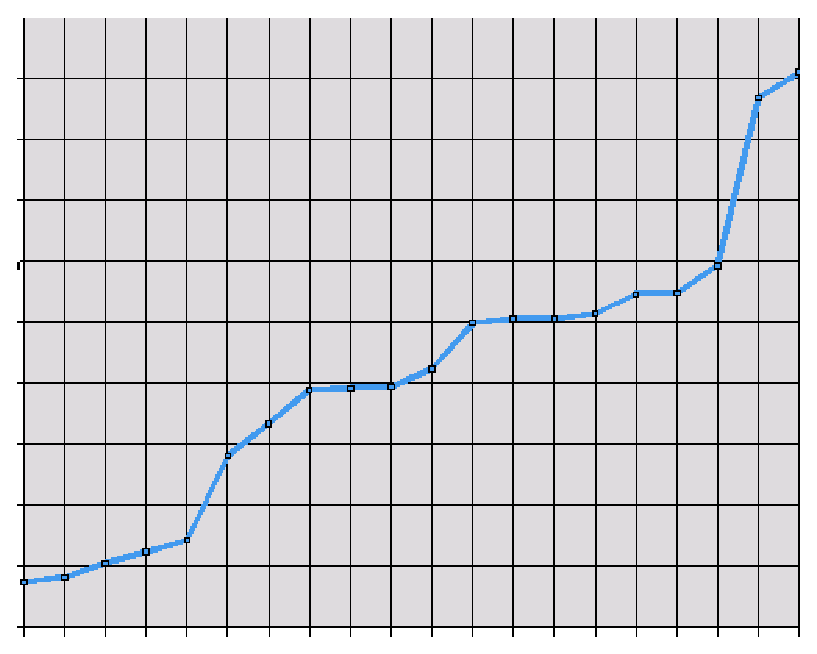
\includegraphics[scale=0.7]{StatistikDia.eps}
	\caption[Diagramm einer statistischen Analyse]{Ein Diagramm aller Entfernungslängen eines \textit{Matches} der Regionen aus \vref{fig:StatistikFla}. Zwischen dem fünften und dem sechsten Wert kann man einen deutlichen Sprung sehen.\\\textit{Quelle: Eigene Darstellung}}
\label{fig:statistik}
\end{figure}

\begin{table}
\caption{Diese Tabelle zeigt alle Entfernungen zwischen den Schwerpunkten der Flächen aus \vref{fig:StatistikFla}. Die Entfernungen, die über der Schwelle, die in \vref{fig:statistik} gefunden wurde, liegen sind markiert.}
\begin{tabular}{|c|c|c|c|c|c|}
\hline
&\textbf{(-103 ; 25)}&\textbf{(-37 ; 55)}&\textbf{(13 ; 73)}&\textbf{(86 ; 43)}&\textbf{(14 ; -14)}\\
\hline
\textbf{(-87 ; 29)}&\textbf{\textit{16,49}}&56,36&109,25&173,57&109,77\\
\hline
\textbf{(-11 ; 67)}&101,13&\textbf{\textit{28,64}}&\textbf{\textit{24,74}}&99,92&84,77\\
\hline
\textbf{(-4 ; -3)}&102,88&66,73&77,88&101,07&\textbf{\textit{21,1}}\\
\hline
\textbf{(79 ; 30)}&182,07&118,66&78,77&\textbf{\textit{14,76}}&78,49\\
\hline

\end{tabular} 
\end{table}


\subsubsection*{\index{Match!Schwellwert}Schwellwertverfahren}\label{Schwellwert}

Das Schwellwertverfahren kann wie folgt formuliert werden: ,,Matche zwei Cycles, wenn der Abstand ihrer Referenzpunkte kleiner als der Schwellwert ist.''

Die Laufzeit dieses Verfahrens ist wesentlich besser. Zu jedem der $m\times n$ verschiedenen  Referenzpunkte wird der  Abstand (in konstanter Zeit) berechnet und mit dem Schwellwert verglichen. Also ist die Laufzeit $O(m\cdot n)$.

Aufgrund der Verschiedenheit der m"oglichen Daten ist ein solcher absoluter Schwellwert $t_{abs}$ nat"urlich nicht handhabbar, so dass die Matchingfunktion mit einem relativen Schwellwert $t_{rel}$ (in \%) arbeiten muss. Aus diesem wird dann intern ein absoluter Schwellwert berechnet, der dann wie oben verwendet wird: Man berechnet $t_{abs}$, indem man $t_{rel}$ mit dem gr"o"sten Abstand multipliziert, den die beiden Regionen voneinander haben. Leider ben"otigt man f"ur die Berechnung dieses Wertes $O(n\cdot m)$. Praktisch wird deshalb ein Algorithmus verwendet, der in $O((n+m)\log{(n+m)})$ einen sehr "ahnlichen Wert berechnet. (Siehe hierzu \vref{maxDist}).

\subsubsection*{Neuronale Netze}\label{neuroNetz}

Man kann die Problematik, Matches von Referenzpunkten zu finden, auch wie folgt beschreiben: In einer Menge von Punkten im $\mathbb{R}^2$ werden Klassen von zusammengehörenden Punkten gesucht.

Solche Klassifizierungsaufgaben sind genau das klassische Einsatzgebiet von neuronalen Netzen. Es steht zu vermuten, dass ein Lernverfahren auf Basis von neuronalen Klassifikatoren sehr gute Ergebnisse liefern wird. 

Auch \textit{Support--Vektor--Maschinen},\index{Support--Vektor--Maschine} wie sie in \cite{SchSm} beschieben werden könnten bei dieser Klassifikation hilfreich sein. Die Idee dieser Maschinen ist es, die Klassifikation durch eine Hyperebene vorzunehmen, deren Rand, in welchem sich keine zu klassifizierenden Objekte befinden, möglichst breit ist. Damit man eine solche Hyperebene benutzen kann, muss der Vektorraum der Objekte in einen geeigneten höherdimensionalen Vektorraum transformiert werden. 

Der Rahmen dieser Arbeit würde aber von beiden Verfahren deutlich überschritten.

\subsection{Beseitigung von 1:n Matches}\label{1zuN}

Der Algorithmus, welcher aus dem Match \textit{MovingSegments} erzeugt, kann ausschließlich mit Matches umgehen, wo es zu jedem Source maximal ein Target gibt. Taucht ein 1:n Matching auf, dann muss dieses aufgel"ost werden. 

\subsubsection*{Alle $\mathbf{n}$ Targets sind Kinder einer einzigen ConvexHullTreeNode}\label{JoinConc}

Gehören alle $n$ Targets zu einem einzigen \textit{ConvexHullTreeNode}, gibt es einen Algorithmus, der schon in \cite{TG} beschrieben wurde, in dem es darum geht, die konvexe H"ulle aller Targets zu bilden und das Matching von den $n$ Targets auf diese neue H"ulle umzuleiten.

Leider versagt dieses Verfahren, falls die gematchten Polygone sich nicht ähnlich genug sind. Es gelang im Rahmen dieser Arbeit leider nicht, das Problem ausreichend einzugrenzen, weshalb auf die Implementierung dieses Verfahrens verzichtet werden musste. Wenn das Verfahren funktioniert, sehen die Ergebnisse aber sehr gut aus. Es erscheint daher lohnenswert, diesem Verfahren weiter nachzugehen.

\subsubsection*{Source ist ein Face oder ein Hole}

Ist die Source--Komponente ein \textit{Face} oder ein \textit{Hole},  so muss der Source aufgeteilt werden. Es wurden einige Überlegungen angestellt, wie es möglich ist, diese Zerteilung möglichst schonend, also ohne dass man das zu teilende Objekt und alle Matches von diesem neu berechnen muss, vornehmen zu können. Die Überlegungen lauten:
\begin{itemize}
\item Ein \textit{ConvexHullTreeNode} ist nur an Eckpunkten oder an Punkten auf Linien zu teilen, die keine Kinder haben, da sonst der \textit{ConvexHullTree} zerst"ort werden.

\item Ein \textit{ConvexHullTreeNode} ist nur an zwei Punkten zu teilen, wenn das beschriebene Polygon auch nur in zwei Teile zerf"allt.

\item Die Zerteilung der Source-Komponente sollte die Lage und das Verh"altnis der Fl"acheninhalte der Target-Komponenten weitestgehend widerspiegeln.

\end{itemize} 

Es wude entschieden diesen schonenden Ansatz nicht weiterzuverfolgen, sondern ein Verfahren zu bnutzen, dass bei dem Zerteilen schönere Ergebnisse findet. Die Nachteile dieses Ansatzes sind die Neuberechnung aller erzeugten Objekte und alle Matches dieser Objekte. Bei der Neuberechnung der neuen Matches ist zu beachten, dass man hier in keine Endlosschleife laufen darf. Eine Endlosschleife kann wie folgt entstehen:

Polygon $A$ wird gegen zwei Polygone $B_1$ und $B_2$ gematcht. Deshalb wird $A$ in $A_1$ und $A_2$ geteilt. Bei der Neuberechnung des Matches wird nun $A_1$ wieder gegen $B_1$  und $B_2$ gematcht. Also muss $A_1$ in $A_{1_1}$ und $A_{1_2}$ geteilt werden, die leider wieder gegen $B_1$ und $B_2$ gematcht werden ...

Um solche Effekte zu umgehen, darf man für $A_1, A_2,B_1$ und $B_2$ nicht ein normales Match berechnen, sondern darf $A_1$ und $A_2$ nur gegen das eine $B_i$ matchen, das am besten passt. 

Wird ein \textit{Face} zerteilt, so kann es passieren, dass dabei ein \textit{Hole} zerteilt wird. Falls sich das nicht verhindern l"asst, zerf"allt das Loch in zwei neue Konkavit"aten, die den neuen \textit{Faces} hinzugefügt werden müssen. Ein Algorithmus, der dieses leistet findet sich unter \vref{JoinLL}. Nichtzerteilte \textit{Holes} müssen demjenigen neuen \textit{Face} zugeordnet werden, in dem diese liegen.

Um ein optisch möglichst ansprechendes Resultat zu erzeugen, müssen sich Form und Lage der Targetobjekte in der Aufsplittung wiederfinden. Ein Algorithmus der dieses liefert, findet sich unter \vref{ZerteilungsAlgo}. Bei diesem Algorithmus gehen nur zwei Polygone auf der Targetseite in die Zerteilung ein. Weitergehende Zersplitterungen lassen sich durch die mehrfache Anwendung dieses Algorithmus erzeugen.

\subsubsection*{Source ist ein untergeordneter ConvexHullTreeNode}

Da man in diesem Fall das oben beschriebene Verfahren nicht anwenden kann, muss man auf folgenden, sehr einfachen Algorithmus zurückgreifen. Dieser  funktioniert analog zu dem Verfahren, mit welchem im letzten Abschnitt Endlosschleifen vermieden wurden.

\par
\begingroup
\leftskip=2em 
Wird $A$ auf  $B_1,B_2, \hdots ,B_n$ gematcht, so lösche alle Matches, außer des einen, welches die höchste Bewertung aus allen Einzelmatches von $A$ auf $B_i$ hat.
\par
\endgroup


Obwohl dieses Verfahren sehr einfach ist, sehen die Ergebnisse überraschend gut aus. Eine Verbesserung könnte hier allenfalls durch den Algorithmus von T\o{}ssebro erreicht werden, wenn man dessen unerwünschte Verhalten abstellen könnte.

\subsection{Beseitigung von "`gedrehten Konkavit"aten"'}\label{gedrehtKon}
In manchen F"allen versagt das in \cite{TG} genannte Verfahren, um aus Matchings \textit{Moving"=Regions} zu erzeugen. Dieses, im Kapitel "`6 Interpolating between two arbitray polygones"' beschriebene Verfahren, setzt voraus, dass die beiden gematchten Kinderpolygone ein gemeinsames, aus zwei Dreiecken zusammengesetztes ,,Trapez'' in der Aussenh"ulle der beiden Vaterpolygone besitzen. 

Dies ist zum Beispiel nicht der Fall, wenn wir uns als Quellpolygon ein "`U"' und als Zielpolygon ein um 90$\degree$ gedrehtes "`U"' vorstellen. Auch wenn die Konkavit"aten richtig zueinander gematcht sind, versagt das bekannte Verfahren.

Die das Matching abschlie"sende Funktion kann solche F"alle erkennen, indem es die Winkel betrachtet, die die gemeinsame Kante von Kind und Vater sowie die beiden Nachbarkanten des Vaters mit der x"~Achse haben. Ist der Winkel der gemeinsamen Kante auf der einen Seite nicht im  Intervall der Winkel der Nachbarkanten der anderen Seite, funktioniert das Verfahren nicht mehr.

\begin{figure}
	\centering
	
\includegraphics[width=.8 \textwidth]{dreh1.eps}
	\caption[Beispiel für gedrehte Polygone]{Beispiel für gedrehte Polygone bei denen das \textit{rotating plane} Vefahren versagt, da die Öffnungen der Konkavitäten kein Trapez bilden.\\\textit{Quelle: Eigene Darstellung}}
	\label{fig:gedrehteMatches}
\end{figure}


Wenn ein solcher Fall erkannt wird, gibt es zwei M"oglichkeiten zu reagieren:
\begin{itemize}
\item Beide Konkavit"aten werden gegen $null$ gematcht

In diesem Fall verschwindet die Konkavit"at auf der einen Seite  und zeitgleich entsteht auf der anderen Seite eine neue. Obwohl dieses Verfahren das deutlich einfachere ist, zeigt sich in der praktischen Anwendung, dass das Resultat den Erwartungen weitestgehend entspricht.

\item Die beiden Konkavit"aten werden zu L"ochern umgewandelt

In diesem Fall werden beide Konkavit"aten in L"ocher verwandelt, die dann zueinander gematcht werden. Im Resultat w"urde sich die Konkavit"at von der einen Seite abl"osen und zu der anderen Seite wandern. M"oglicherweise sieht dieses Verfahren nat"urlicher aus, es ist aber nicht absehbar, was passiert, wenn der Weg zwischen den beiden Positionen nicht "`frei"' ist (etwa weil sich hier ein weiteres Loch oder eine Konkavit"at befindet). Aus diesen Gründen wurde das erste Verfahren implementiert.
\begin{figure}
	\centering
	
\includegraphics[width=.8 \textwidth]{dreh2.eps}
	\caption[Schnappschüsse von gedrehten Polygonen]{Zwei Schnappschüsse von dem \textit{Match} aus Abbildung~\vref{fig:gedrehteMatches}, in dem die Konkavitäten gegen $null$ gematcht wurden.\\\textit{Quelle: Eigene Darstellung}}
	\label{fig:gedrehteMatches2}
\end{figure}

\end{itemize}


\subsection{\index{Match!optimales}Erstellung eines Matches aus mehreren anderen}\label{bewertung}


Es ist festzustellen, dass unter der Betrachtung der bereits erstellten Matchings das Overlapping--Match besser auf Vereinigungen und Aufsplitterungen von \textit{Cycles} reagiert und dass das Schwerpunkt-Verfahren besser auf kleine und schnelle \textit{Cycles} abgestimmt ist. 

Es scheint also ein verfolgenswerter Ansatz zu sein, beide Matches (und vielleicht noch andere, etwa Overlapping mit mehreren Schwellwerten) zu berechnen und aus diesen das beste Matching zu bestimmen. 

Zur Bestimmung der G"ute eines gegebenen Matchings sind nachfolgende Verfahren angedacht. Damit die verschiedenen Bewertungen vergleichbar sind, sind diese auf 1 normiert.

\begin{enumerate}
\item Die \index{Bewertung!Overlap}Overlap-Bewertung: 

Ein gro"ser Durchschnitt der "Uberlappungen wirkt sich positiv auf die Bewertung aus.

Dieses Bewertungsverfahren korrespondiert zwar direkt mit dem Overlapping--Match und ist deshalb als alleiniges Vergleichskriterium abzulehenen. Trotzdem wird es in dieser Arbeit als einer von mehrere Bewertungsansätzen benutzt, da die Überlappung sich als sehr interessantes Kriterium erwiesen hat. Die Berechnung l"auft so:

$$r_O=\frac{\sum_{m\in M} \frac{A_{overlap}}{A_{source}+A_{target}}}{|M|}$$

\item Die \index{Bewertung!Hausdorff}Hausdorff-Bewertung:

In \cite{AAR} wird die oben bereits eingef"uhrte, Hausdorff-Norm benutzt, um Matchings zu bewerten. 

Bei der Implementierung dieser Norm stellt sich die Frage der Normierung. Mangels Alternative werden alle einzelnen Hausdorff--Abst"ande durch den Duchmesser $d$ der Ausgangsregionen geteilt.  Durchmesser bezeichnen hierbei den gr"o"sten Abstand, den zwei Punkte zueinander haben. Dieses Vorgehen bedeutet aber leider, dass die Abst"ande von kleinen Konkavit"aten relativ wenig in die Gesamtbewertung eingehen. Die Berechnung lautet:

$$r_H=\frac{1}{|M| \cdot d}\sum_{m\in M}\delta_H(m)$$

\item Die Bewertungen durch Minimierung einer Norm über geeignete Abbildungen

\cite{AAR} und \cite{AFRW} enthalten beide die Bewertung:
$$\min_{T\in\mathcal{T}}\: \delta(A,T(B))$$
$\delta$ kann hierbei entweder der Hausdorff-Abstand oder die symmetrische Differenz sein. Das Problem an diesem Ansatz ist die Berechnung der minimierenden Abbildung $T$. Algorithmen zur Findung dieser Abbildung werden zwar angegeben, die Implementierung dieser würden aber den Umfang dieser Arbeit sprengen.

\item Die \index{Bewertung!Referenzpunkt}Referenzpunkt-Bewertung:

Ein kleiner Durchschnitt der Entfernungen der zueinander gematchten Referenzpunkte wirkt sich positiv auf die Bewertung aus.

Da dieses Verfahren direkt mit dem Schwerpunkt-Match bzw. dem Steinerpunkt"=Match korrespondiert und außerdem nach \cite{AFRW} und \cite{AAR} nicht zu erwarten steht, dass dieses Verfahren deutlich andere Werte als die Overlap-Bewertung bzw. die Hausdorff-Bewertung liefert, wird dieses nicht weiter verfolgt.

\item Die \index{Bewertung!Flächensummen}Summen-Bewertung:


Etwa gleich gro"se, zueinander gematchte Fl"achen wirken sich positiv auf die Bewertung aus.

Es steht zu erwarten, dass zueinander geh"orige Fl"achen etwa gleich groß sind. Auch wenn sich eine Fl"ache in mehrere andere teilt, wird die Summe der Fl"acheninhalte in etwa so gro"s sein wie der Fl"acheninhalt der Ursprungsfl"ache. Zur Normierung teilt man den kleineren durch den gr"o"seren Fl"acheninhalt und bekommt somit die Abweichung in Prozent. Die Berechnung l"auft nach folgender Formel:

$$A_{target}=\sum_{t\in Target}A_t$$
$$r_A=\frac {\sum_{m\in M}\frac{\min({A_{source},A_{target}})}{\max({A_{source},A_{target}})}}{|M|}$$



\item Die \index{Bewertung!linear}Linear-Bewertung:

Bei der Implementierung der obigen Verfahren zeigte sich, dass die Verfahren eine Tendenz zu "ubertriebenen Zersplitterungen aufweisen. Unter der Pr"amisse, dass dies in den allermeisten F"allen eher unerwünscht ist, wurde dieser Bewertungsfaktor eingef"uhrt, um dieses Verhalten abzuschw"achen.

F"uhrt das Matching zu einer geringen Anzahl an Zersplitterungen, wirkt sich das positiv auf die Bewertung aus.

Die Berechnung l"auft gemäß:

$$L(m)=
\begin{cases}
	\frac{1}{2} & \text{falls }|targets|=0\\
	\frac{1}{|targets|} & \text{sonst}
    \end{cases}
$$

$$r_L=\frac{\sum_{m\in M}L(m)}{|M|}$$

\item Die \index{Bewertung!strukturell}Struktur-Norm:

Stimmen die aufeinander gematchten \textit{Cycles} strukturell weit "uberein, wirkt sich das positiv auf die Bewertung aus. Eventuell kann man hier die Struktur der jeweiligen ConvexHullTrees heranziehen.

Diese Norm wird im Rahmen der vorliegenden Arbeit nicht weiterverfolgt, bietet aber möglicherweise einen interessanten Anknüpfungspunkt für künftige Untersuchungen. Zur Struktur der ConvexHullTrees ist zu sagen, dass in \cite{TG} der Umstand beschrieben ist, dass "ahnliche Polygone teilweise recht unterschiedliche ConvexHullTree-Repr"asentationen aufweisen k"onnen, was eine solche Bewertung nat"urlich negativ beeinflussen kann\footnote{Herr T\o{}ssebro macht aber in diesem Artikel plausibel, dass dieses Problem eher ein Problem von kleinen, k"unstlichen Testdatens"atzen als von realen Daten ist.}.


\end{enumerate} 

Wie man am Beispiel der Summen-Norm sehen kann, gibt es mehr M"oglichkeiten zu bewerten als es effiziente Matchings gibt. Das Summen-Matching, das lauten k"onnte, "`Matche ein Cycle mit  einer Menge von anderen, wenn die Summe der Fl"acheninhalte fast gleich ist zu dem Fl"acheninhalt des Cycles"', entspricht dem Rucksack-Problem und ist daher nicht effizient l"osbar. Die Bewertung, wie gut ein gegebenes Matching ist, ist mit diesem Verfahren aber effizient m"oglich.

\index{Rucksackproblem}Bei einer Variante des Rucksackproblems geht es um die Frage, ob sich eine Zahl $c$ aus einer Teilmenge von gegebenen Zahlen $C=\{c_1,c_1,\hdots,c_n\}$ additiv zusammensetzen läßt. Also 
 $$\exists \tilde{C}\subset C$$ 
$$\sum_{i=0}^{|\tilde{C}|} c_i\quad = c.$$ Beschrieben wird dieses Problem in \cite{Ruck}.

\section{Gemeinsame Grundlagen}

\subsection{Beschreibung von verwendeten Algorithmen} \label{Algorithmen}
In diesem Abschnitt werden Algorithmen vorgestellt, die entweder sehr zentral f"ur die L"osung des Interpolationsproblems oder die keine Standard-Algorithmen sind. Diese Algorithmen müssen demnach selbst entwickelt werden.

\subsubsection{\index{Hashwerte!Berechnung}Effiziente Berechnung von Hashwerten aus \textit{RegionTreeNodes}}\label{berechenHashwerte}

Um \textit{RegionTrees} als Schlüssel in der Hash-Table benutzen zu können, muss aus diesen ein Hashwert berechnet werden können. In die Berechnung des Hashwertes muss jede einzelne Ecke des RegionTrees eingehen. Damit ist die Ermittlung dieses Wertes leider eine aufwendige Operation, zumal auf diesen Wert im Verlauf eines Matching-Verfahrens sehr oft zugegriffen werden muss. Deshalb ist es sinnvoll, die Hashwerte dieser Objekte zu cachen. 

Um sicherzustellen, dass ein Hashwert immer aktuell ist und keine überflüssigen Neuberechnungen notwendig sind, wurde ein Cachingverfahren gewählt, das analog zu einem bekannten Verfahren aus der technischen Informatik abläuft. Jedes Objekt des RegionTrees verfügt über ein ,,Dirty-Flag''. Dieses Flag gibt an, ob der gecachte Wert noch aktuell ist. Es wird bei jeder Operation gesetzt, die das Objekt so verändert, dass sich der Hashwert auch ändern müsste. Bei jedem lesenden Zugriff auf den Hashwert wird 
\begin{itemize}
\item der gecachte Wert zurückgegeben, falls das Dirty-Flag nicht gesetzt ist.
\item Ist das Dirty-Flag gesetzt, so wird der Hashwert neu berechnet, das Dirty-Flag gelöscht und der neuberechnete Wert zurückgegeben.
\end{itemize}

Beim Setzen des Dirty-Flags ist darauf zu achten, dass auch bei dem Vaterelement und allen Vorfahren des Vaterelements dieses gesetzt werden muss.

Dieses Verfahren stellt sicher, dass die Berechnung des Hashwertes wirklich nur dann erfolgt, wenn dies notwendig ist.

Die Berechnung geht wie folgt vonstatten:

\begin{itemize}
\item Konvexer Hüllenbaum

Die Berechnung startet mit einem zufällig  gewählten, fixen Wert. Zu diesem wird dann die kumulierte Summe gebildet, $HV=\lfloor HV+x_i*321+y_i*321\rfloor$. Die Zahl 321 ist wieder willkürlich gewählt. Da sich aber geographische Koordinaten oft nur wenig unterscheiden und eine Unterscheidung, etwa von Dreiecken, die nahe beieinander liegen, gewährleistet sein muss, darf dieser Wert nicht zu klein gewählt sein. 

In die Berechnung geht auch noch ein Vielfaches der Ebene ein, auf der sich der Konten in dem Baum  befindet. Außerdem geht noch eine feste Zahl ein, die nur zum Tragen kommt, falls das Objekt ein \textit{Hole} ist.

\item Face

Der Wert für ein \textit{Face} wird berechnet, indem man zu dem Hashwert des \textit{Cycles} alle Hashwerte der Löcher hinzuaddiert. Dem Ergebnis wird noch ein weiterer, konstanter Summand hinzugefügt. Dadurch ist sichergestellt, dass der Hashwert eines \textit{Faces}, welches nur aus einem einzigen \textit{Cycle} besteht, sich von dem Hashwert des \textit{Cycles} unterscheidet.

\item Region

Der Hashwert einer \textit{Region} setzt sich wiederum aus den Hashwerten seiner \textit{Faces} und einem weiteren konstanten Summanden zusammen.
\end{itemize}
\newpage
\subsubsection{\index{splitline}Berechnung einer Zerlegungslinie für einen \textit{ConvexHullTreeNode} aus zwei anderen}\label{ZerteilungsAlgo}

Dieser Algorithmus bekommt ein zu zerteilendes ConvexHullTreeNode ($A$) und zwei andere ConvexHullTreeNodes ($B_1$ und $B_2$). Berechnet werden soll nun ein Linienzug, der die Lage und Form von $B_1$ und $B_2$ möglichst gut wiedergeben soll und an dem sich $A$ zerteilen lassen kann.

Die weitere Besprechung dieses Algorithmus wird am Beispiel von drei Polygonen vorgenommen. Diese drei sind in Abbildung~\vref{fig:ZuZersplitten} zu sehen.

\begin{figure}
	\centering
	\includegraphics[scale=0.45]{ZuZersplitten.eps}
	\caption[Zu teilendes Polygon mit Referenzpolygonen]{Die Polygone $A$ (gelb), $B_1$ (blau) und $B_2$ (rot).\\\textit{Quelle: Eigene Darstellung}}
	\label{fig:ZuZersplitten}
\end{figure}

Zuerst werden die Schwerpunkte $M_1$ und $M_2$  von $B_1$ und $B_2$ berechnet. Dann werden die Eckpunkte der beiden Polygone nach solchen Punkten gefiltert, die auf einer Orthogonalen zu der Strecke zwischen $M_1$ und $M_2$ liegen. Die beiden Ergebnislisten werden nach dem Abstand von dem Punkt zur Linie zwischen $M_1$ und $M_2$ sortiert, wobei die Abstände auf einer Seite der Linie negativ gewertet werden.

Die beiden Listen der Endpunkte zeigen für das Beispiel die folgende Tabellen. Abbildung~\vref{fig:RectDist} zeigt die entsprechenden Punkte grafisch.

\begin{table}[!h]
\begin{tabular}{|c|r|r|r|r|r|r|r|r|}
\hline
Punkt&
 102&
 103&
 104&
 106&
 105&
 107&
 108&
 109\\
\hline
Entfernung&
   88&
   44&
   35&
   16&
   -1&
  -29&
  -49&
 -111\\
\hline
\end{tabular} 
\caption{Die Punkte von $B_1$}
\end{table}
\begin{table}[!h]


\begin{tabular}{|c|r|r|r|r|r|r|r|}



\hline
Punkt&
 206&
 205&
 204&
 203&
 202&
 201&
 200
\\
\hline
Entfernung&
   75&
   42&
   25&
  -18&
  -42&
  -63&
 -121
\\
\hline
\end{tabular} 
\caption{Die Punkte von $B_2$}
\end{table}


\begin{figure}
	\centering
	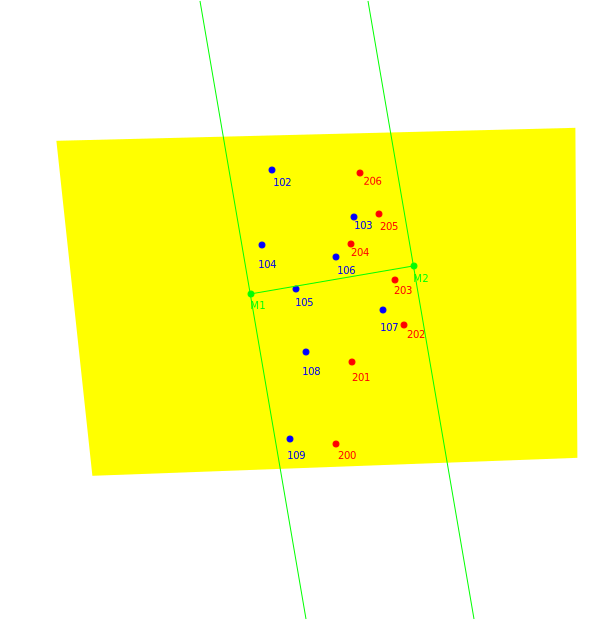
\includegraphics[scale=0.5]{RectDist.eps}
	\caption[Punkte mit einem rechtwinkeligen Abstand zur Schwerpunktlinie]{Alle Punkte von $B_1$ und $B_2$, die in dem Streifen zwischen den beiden Schwerpunkten von $B_1$ und $B_2$ (namens $M_1$ und $M_2$) liegen.\\\textit{Quelle: Eigene Darstellung}}
	\label{fig:RectDist}		
\end{figure}


Nun nimmt man aus jeder Liste die beiden oberen Punkte und betrachtet die Linie zwischen diesen Punkten. Schneidet diese Linie keines der beiden Polygone (außer an den Endpunkten), merkt man sich den Mittelpunkt der Linie in der neuen Liste  $Mittelpunktlinie$. Aus den Listen wird nun der größere der beiden Punkte gelöscht, falls dieser nicht der letzte in der Punktliste ist. Dieses Vorgehen wird solange fortgesetzt, bis beide Listen nur noch ein einziges Element haben. Die fiktiven Verbindungslinien und ihre Mittelpunkte sind in Abbildung~\vref{fig:Mittelpunkte} zu sehen.

\begin{figure}
	\centering
	\includegraphics[scale=0.6]{Mittelpunkte.eps}
	\caption[Verbindungslinien und deren Mittelpunkte]{Alle gefilterten Punkte aus $B_1$ und $B_2$, die zulässigen Verbindungslinien und deren Mittelpunkte.\\\textit{Quelle: Eigene Darstellung}}
	\label{fig:Mittelpunkte}
\end{figure}

Der Linienzug, der sich nun aus der Liste $Mittelpunktlinie$ ergibt, liegt genau zwischen den beiden Polygonen und bildet die Struktur der Polygone an der Stelle ab, an der die beiden Polygone einander zugewandt sind. Dieser Linienzug ist in Abbildung~\vref{fig:MittelpunktLinie} zu sehen.

\begin{figure}
	\centering
	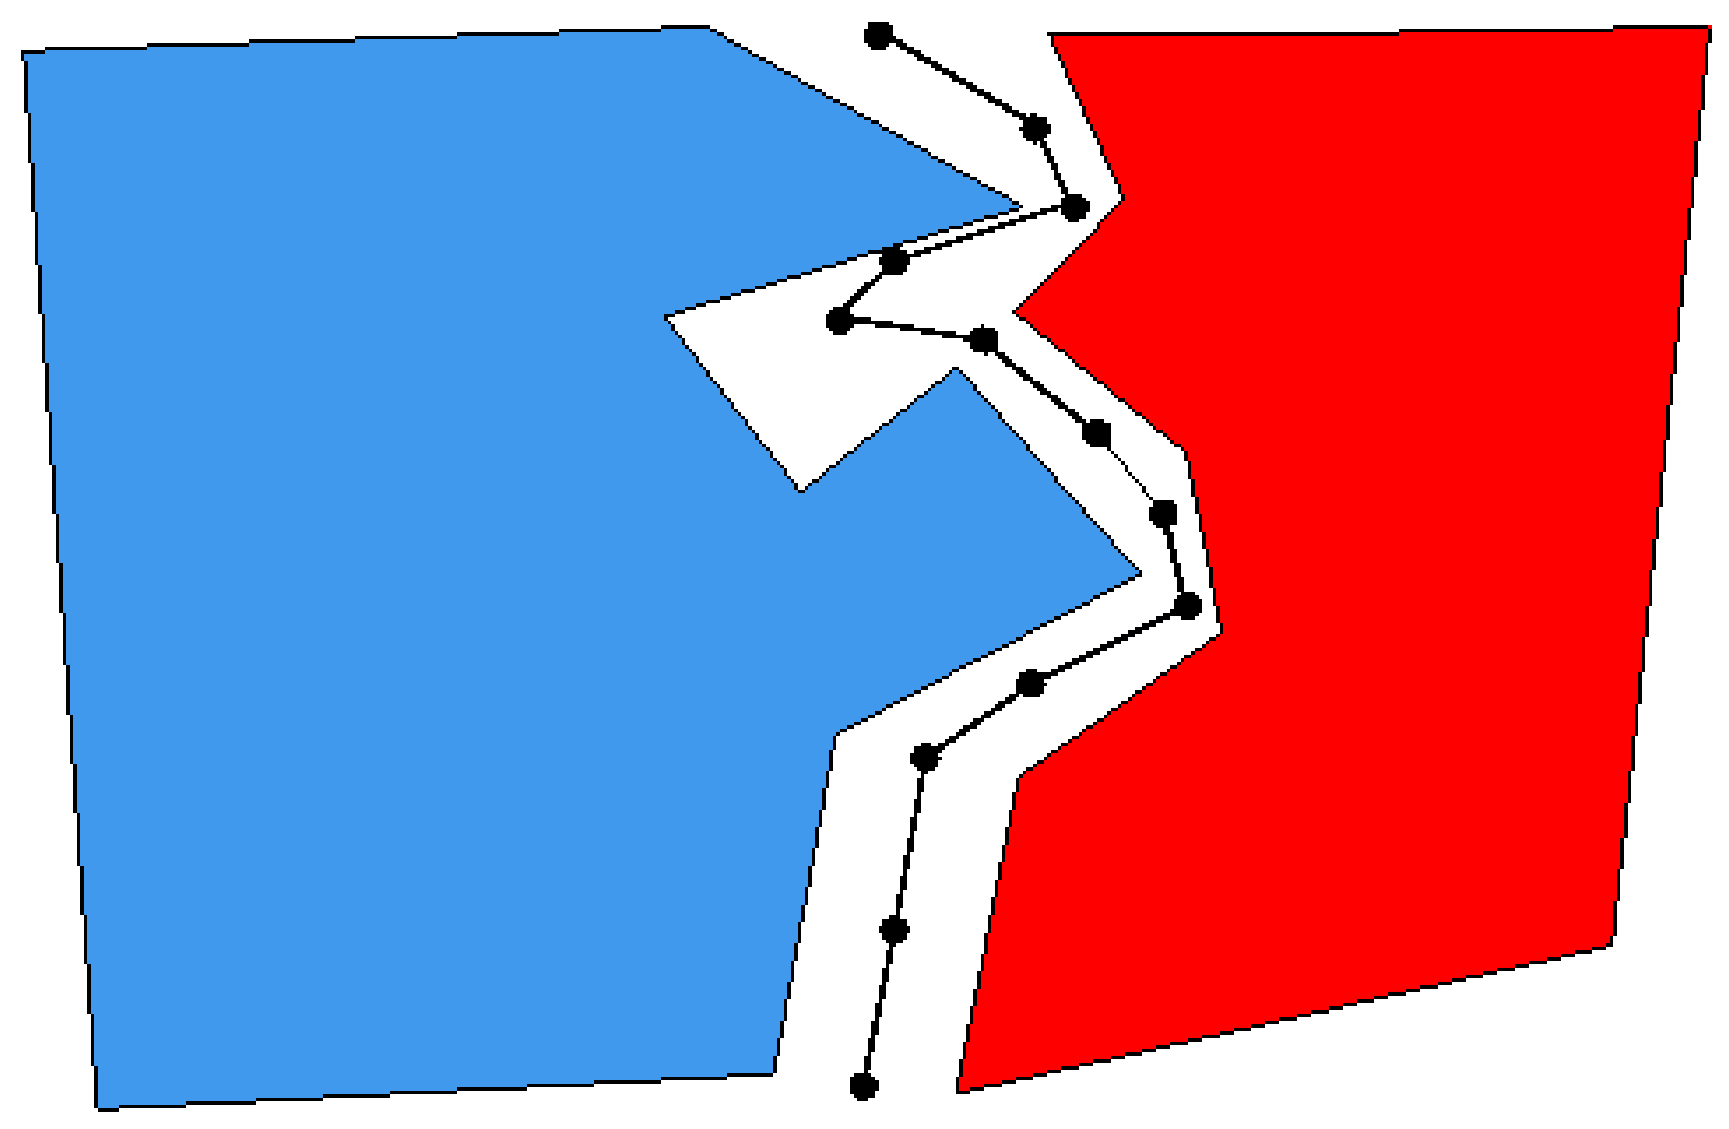
\includegraphics[scale=0.4]{MittelpunktLinie.eps}
	\caption[Polygone mit dem berechneten Linienzug]{$B_1$ und $B_2$ mit dem berechneten Linienzug.\\\textit{Quelle: Eigene Darstellung}}
	\label{fig:MittelpunktLinie}
\end{figure}

In der Regel teilt diese Linie aber nicht $A$, wie man an dem Beispiel gut sehen kann. Damit diese Linie nun wirklich durch $A$ geht, $A$ komplett geteilt wird und die Lage von $B_1$ und $B_2$ trotzdem noch widergespiegelt werden, sind folgende Schritte durchzuführen:

\begin{enumerate}
\item Berechne die Schwerpunkte $M_L$ der Linieneckpunkte, $M_A$ von $A$ und $M_B$ aller Eckpunkte von $B_1$ und $B_2$.
\item Berechne den Skalierungsfaktor $s_1=\frac{|A|}{|B_1|+|B_2|}$. 
\item Berechne das Maximum der Entfernungen $d_L$ von $M_L$ zu den beiden Endpunkten des Linienzuges 
\item Berechne die maximale Entfernung $d_A$ von $M_A$ zu den Eckpunkten von $A$.
\item Berechne den Skalierungsfaktor $s_2=\frac{d_A}{d_l} * 1,05$. Die 5\% sind willkürlich gewählt und sollen die Wahrscheinlichkeit erhöhen, dass beide Endpunkte des neuen Linienzuges außerhalb von $A$ liegen. 5\% haben sich in praktischen Versuchen bewährt.
\item Berechne den neuen Linienzug $l'_1,l'_2,\hdots ,l'_n$ durch $\:l'_i=M_A+(l_i-M_l)*s_1+(M_l-M_B)*s_2$.
\end{enumerate}


Abbildung~\vref{fig:SplitLine} zeigt das Ergebnis dieses Beispiels. 

Wie man schon an dem willkürlichen Faktor 5\% sehen kann, liefert dieser Algorithmus nicht in allen Fällen ein zulässiges Ergebnis. Die Erfolgsquote scheint aber sehr hoch zu liegen, in allen Beispielen, die im Laufe der Entwicklung aufgelaufen sind, tauchte kein einziger Fall auf, wo der Split versagte. Die Ergebnisse sahen auch alle sehr natürlich aus.


\begin{figure}
	\centering
	\includegraphics[scale=0.6]{Ergebnis.eps}
	\caption[Polygon mit der berechneten SplitLine]{Das Polygon $A$ mit der berechneten \textit{SplitLine}.\\\textit{Quelle: Eigene Darstellung}}
	\label{fig:SplitLine}
\end{figure}

\clearpage
\subsubsection{Zerteilte Löcher als Konkavitäten in ein \textit{Cycle} einbauen}\label{JoinLL}

Wenn durch die Teilung eines \textit{Faces} auch die Teilung eines \textit{Holes} verursacht wird, so werden aus den beiden neuen Polygonen Konkavitäten in den beiden neuen \textit{Faces}. Zunächst muss jede dieser Konkavitäten dem passenden \textit{Face} zugeordnet werden. Hierzu sucht man einen Punkt des neuen Polygons, der nicht auf dem Rand eines \textit{Faces} liegt. Das passende \textit{Face} ist dann dasjenige, in welchem der gewählte Punkt liegt. 

Als Beispiel betrachten wir das Polygon $A$ aus dem letzten Abschnitt als \textit{Face} und ergänzen dieses durch ein \textit{Hole}. Als Schnittlinie wird die eben berechnete benutzt (siehe Abbildung~\vref{fig:JLL1}).

\begin{figure}
	\centering
	\includegraphics[width=0.5\textwidth]{JLL1.svg.eps}
	\caption[Face mit einem Hole wird geteilt]{$A$ aus dem letzten Beispiel, jetzt um ein zu teilendes \textit{Hole} ergänzt.\\\textit{Quelle: Eigene Darstellung}}
	\label{fig:JLL1}
\end{figure}

Der Algorithmus zum Vereinigen der Polygone bekommt nun also zwei Polygone als geordnete Listen von Eckpunkten, das neue Face und ein passendes Bruchstück eines Holes. Diese Punktlisten werden zunächst sortiert. Die Punkte des Face werden wie gewöhnlich gegen den Uhrzeigersinn  angeordnet, die des Holes hingegen im Uhrzeigersinn. Zunächst wird  ein Punkt auf dem Rand des Faces gesucht, der nicht auf dem gemeinsamen Rand von Hole und Face liegt. Im Beispiel wird Punkt 0 gewählt.

Jetzt werden die Punkte des Faces durchgegangen, solange auf der Linie zwischen dem aktuellen Punkt und dem nächsten kein Punkt des Holes liegt. All diese Punkte werden der Ergebnisliste $res$ hinzugefügt.

Also: $res=(0, 1, 2, 3, 4, 5)$.

Dann wird aus allen Punkten des Holes, die auf der Linie von 5 zu 6 liegen, der Punkt, der am nächsten zu 5 liegt,  gesucht. Im vorliegenden Fall ist das 107, der wieder an $res$ anhänget wird. Dieses etwas kompliziert klingende Vorgehen deckt eine Reihe von Sonderfällen ab, die hier auftauchen können. Abbildung~\vref{fig:SonderfaelleJLL} zeigt diese exemplarisch.

$res=(0, 1, 2, 3, 4, 5, 107)$

Nun werden die Punkte des Holes,  mit 100 beginnend, solange durchlaufen, bis der aktuelle Punkt auf dem Rand des Faces liegt (hier 103). Alle besuchten Punkte werden an $res$ angehängt.

Daraus folgt: $res=(0, 1, 2, 3, 4, 5, 107, 100, 101, 102, 103)$

Anschließend wird wieder das Face durchlaufen, wobei bei 6 begonnen wird. Es wird  der erste Punkt  gesucht, der nicht auf dem Hole liegt. Im Beispiel ist dies Punkt 9.

Abschließend werden an $res$ alle Punkte angehängt, bis der Ausgangspunkt wieder erreicht wird.

Schließlich ist $res=(0, 1, 2, 3, 4, 5, 107, 100, 101, 102, 103, 9, 10, 11, 12)$. Abbildung~\vref{fig:JLL3} zeigt das Ergebnis als Polygon.


\begin{figure}
	\centering
	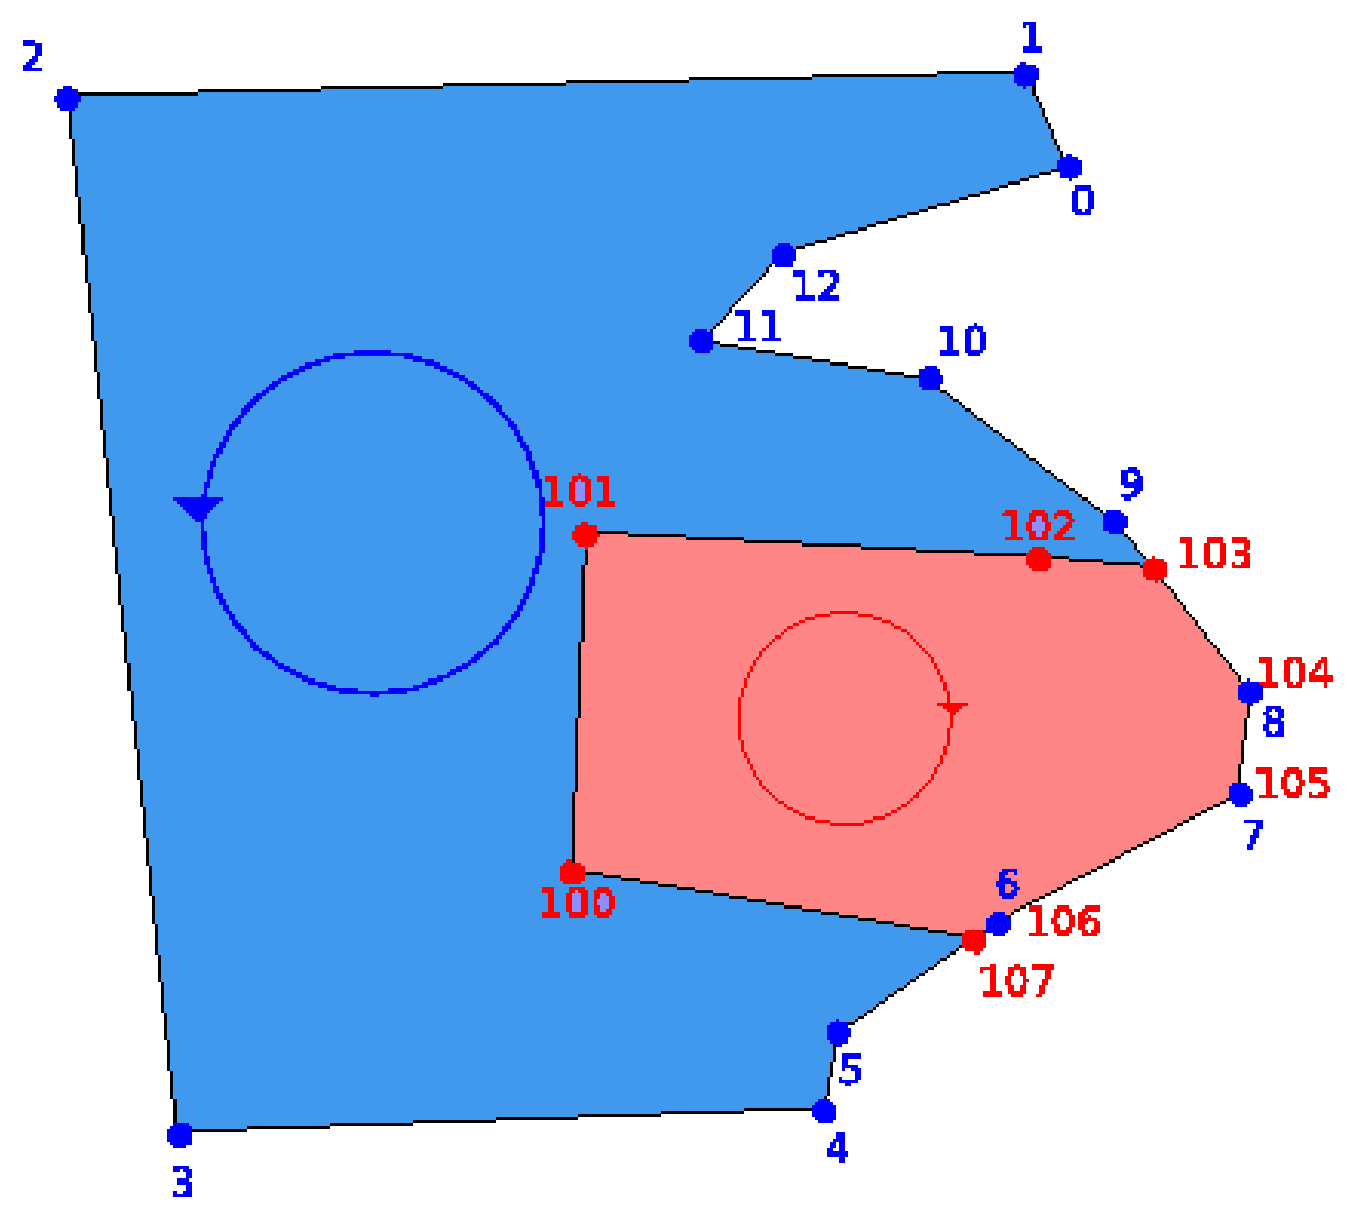
\includegraphics[width=0.5 \textwidth]{JLL2.svg.eps}
	\caption[Verbindung zweier Polygone] {Die beiden neu entstandenen Polygone sollen verbunden werden.\\\textit{Quelle: Eigene Darstellung}}
	\label{fig:JLL2}
\end{figure}


\begin{figure}
\subfigure[Beide Berührungspunkte liegen auf der selben Facelinie.]{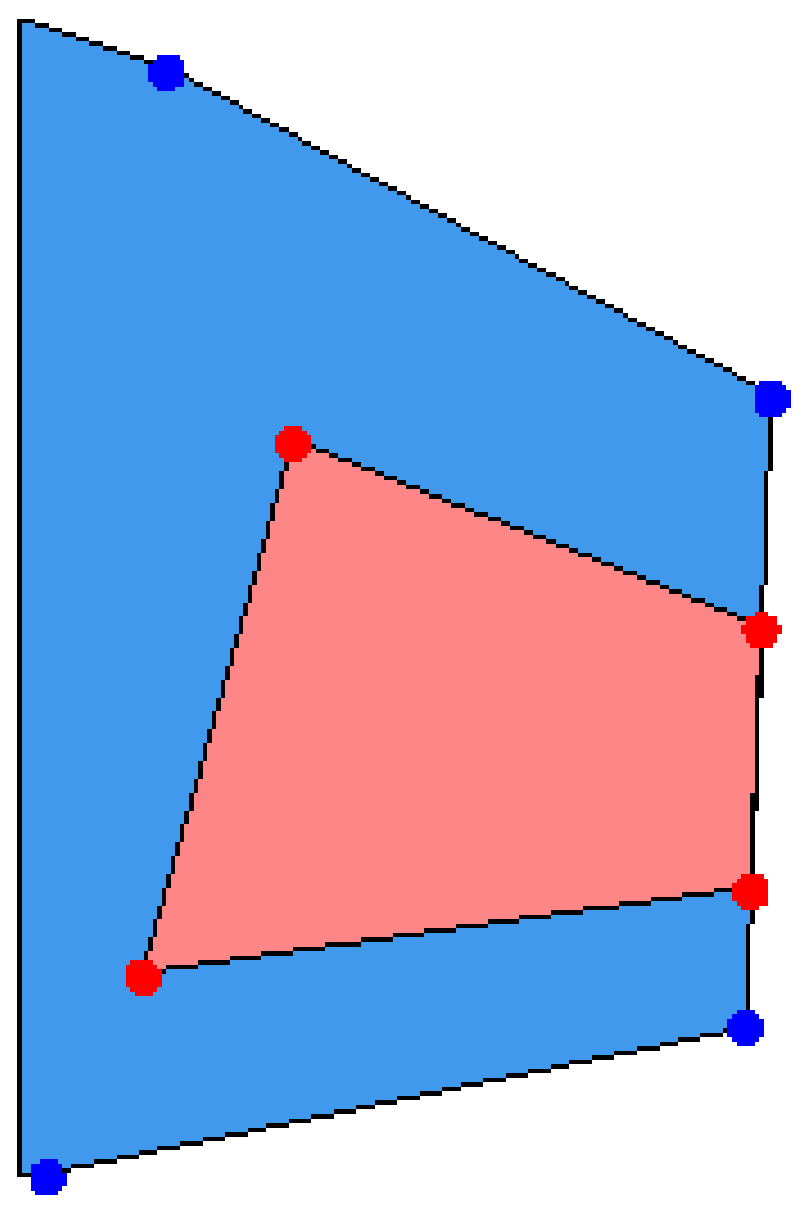
\includegraphics[width=0.35\textwidth]{Sonderfall1JLL.svg.eps}}\hfill
\subfigure[Der erste Punkt des Holes ist auch ein Punkt des Faces]{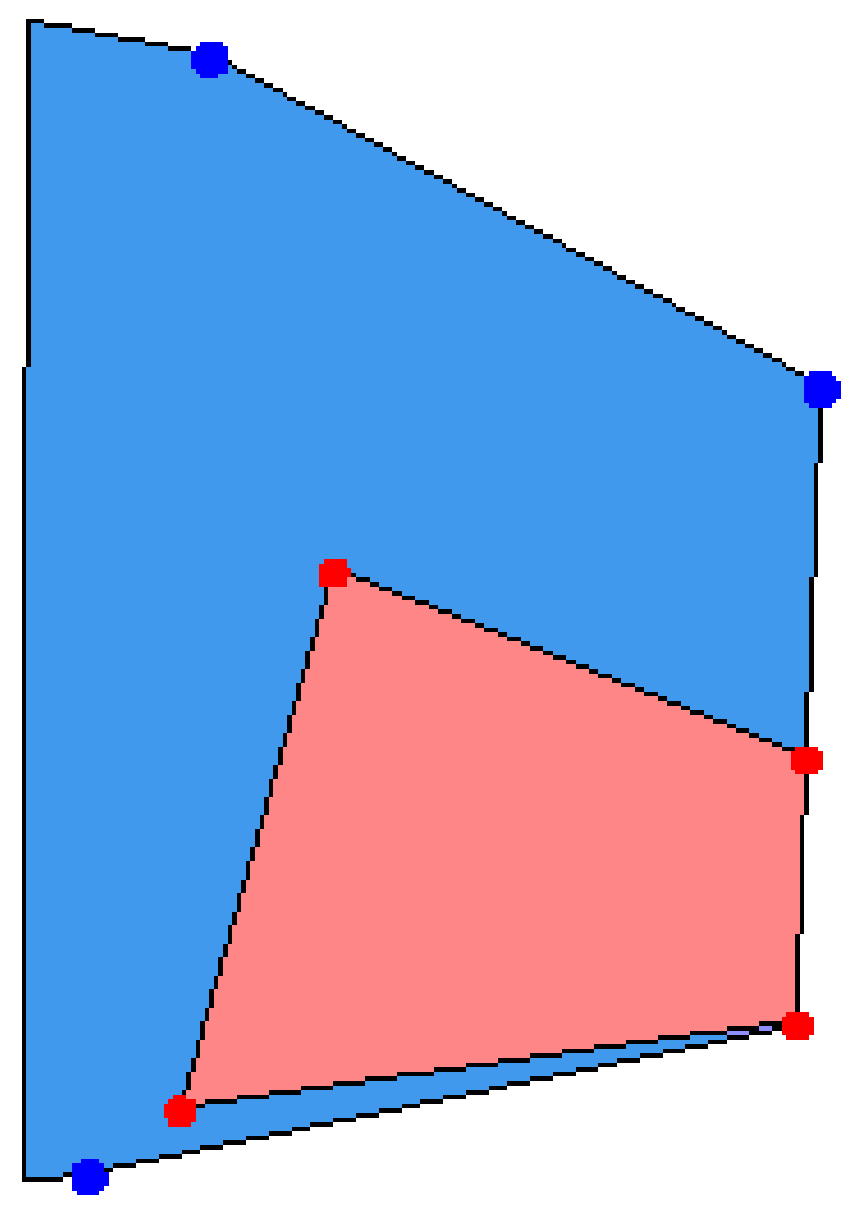
\includegraphics[width=0.35\textwidth]{Sonderfall2JLL.svg.eps}}
\caption[Sonderfälle die bei der Vereinigung auftreten können]{Sonderfälle, die bei der Vereinigung auftreten können und wegen denen man die Funktion \textit{getClosestBoundaryPoint} benötigt.\\\textit{Quelle: Eigene Darstellung}}
\label{fig:SonderfaelleJLL}
\end{figure}



\begin{figure}
	\centering
	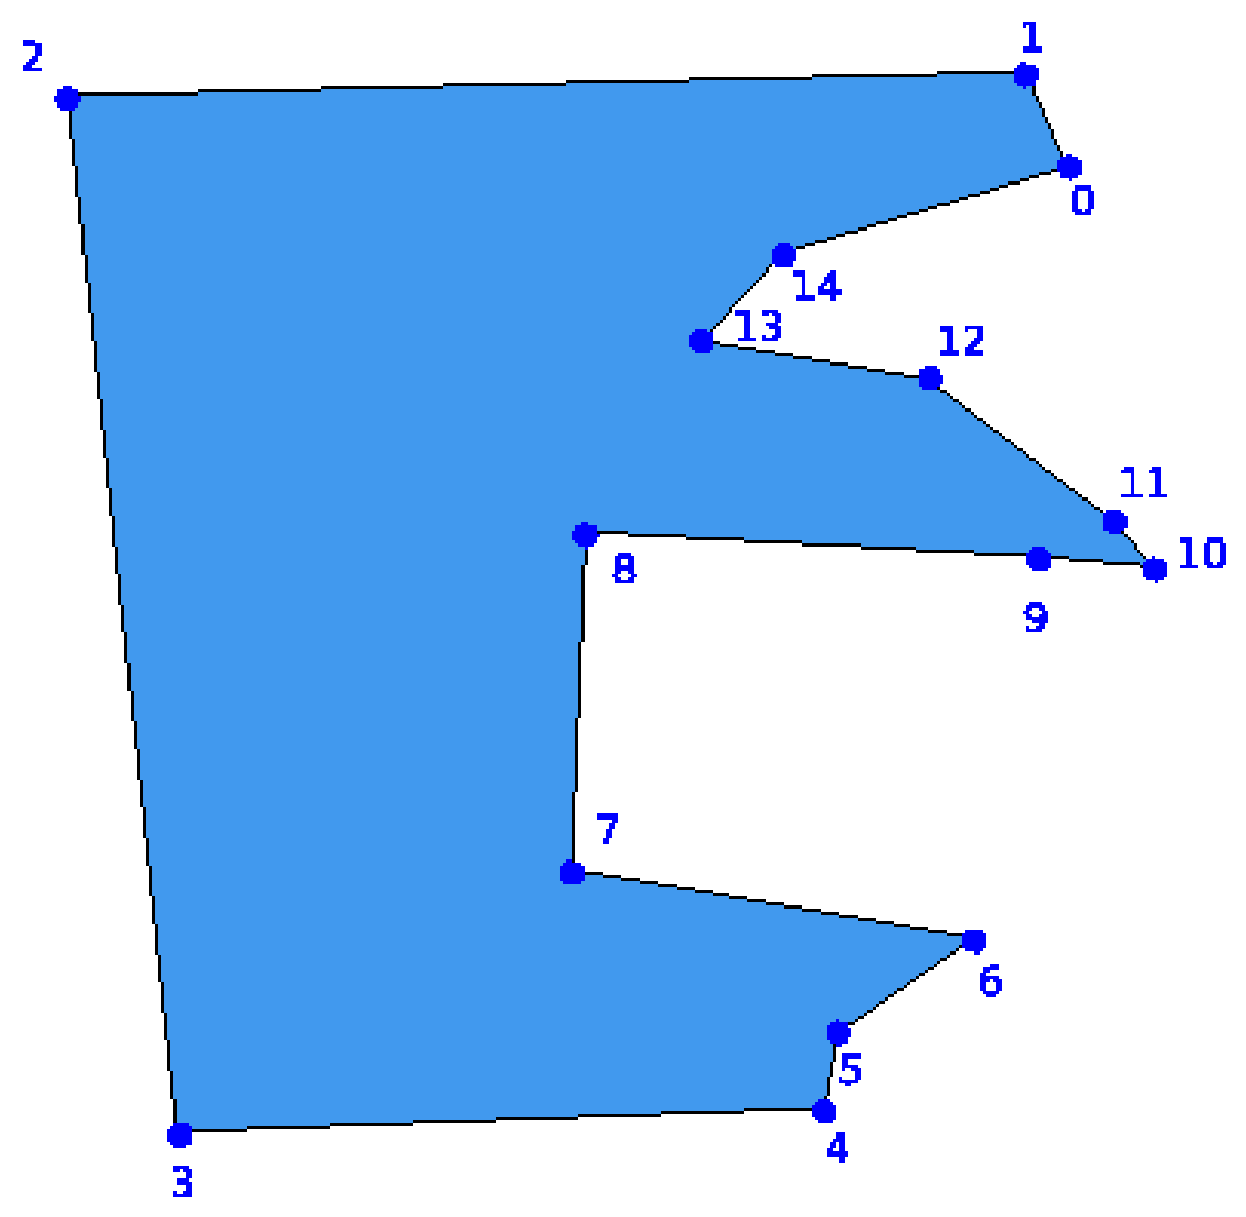
\includegraphics[width=0.6\textwidth]{JLL3.svg.eps}
	\caption[Fertig zusammengesetztes Polygon]{Das fertig zusammengesetzte Polygon.\\\textit{Quelle: Eigene Darstellung}}
	\label{fig:JLL3}
\end{figure}


\clearpage
\subsubsection{\index{Rotaring Plane}Rotating Plane} \label{rotPane}
In \cite{TG} wurde bereits der Algorithmus ,,rotating Plane'' vorgestellt. Im Laufe der vorliegenden Arbeit wurde eine andrere Implementierung dieses Algorithmus entwickelt und hierbei eine Version gefunden, die sowohl einfacher ist als auch erheblich weniger Fallunterscheidungen benötigt.

Die Idee dieses Algorithmus ist es, zu jeder Kante den Winkel zu bestimmen, den dieser mit der x"~Achse bildet. Zu zwei Ecken, die sich eine gemeinsame Kante teilen, konstruiert man ein Dreieck mit dem Startpunkt der Kante des anderen Polygons, dessen Winkel zwischen den Winkeln des Startpolygons liegt.

\begin{figure}
\centering
\subfigure[Zwei Vierecke, die als Beispiel betrachtet werden.]{\includegraphics[width=0.4\textwidth]{RotatingPlane2.svg.eps}}
\subfigure[Die Tabelle zeigt welche Kanten auf welche Ecken gematcht werden.]{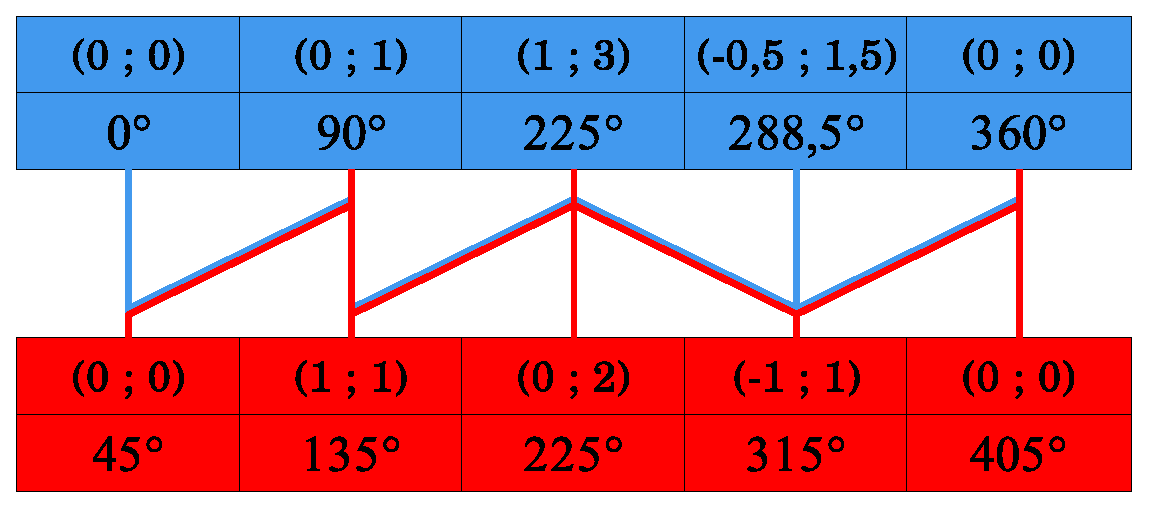
\includegraphics[width=0.7\textwidth]{RotatingPlane.eps}}
	\caption[Tabellendarstellung des rotating Plane]{Diese Abbildung zeigt die beiden Felder zweier Vierecke und zeigt, welche Punkte zusammen ein \textit{MovingSegment} bilden.\\\textit{Quelle: Eigene Darstellung}}
	\label{fig:RotatinPane}
\end{figure}


Hierzu werden zwei Felder von Punkten gebildet, für jedes Polygon eines. Zu jedem Punkt wird dann der Winkel hinzugefügt, den die Linie mit der x"~Axhse hat, welche von diesem Punkt ausgeht. Die einzelnen Elemente dieses Feldes sind Objekte der Klasse \textit{LineWA}. Diese Klasse, die unter \vref{LineWA} dargestellt wird, ermöglicht die Verwaltung eines Punktes mit einem Winkel.  Die Felder werden dann nach diesem Winkeln sortiert. Zu zwei aufeinanderfolgenden Punkten des ersten Polygons wird dann der passende Punkt aus dem zweiten Polygon gesucht. Hierzu wird die Funktion \textbf{finde\_passenden\_Index()} benutzt, die weiter unten erklärt wird. Das so entstandene Dreieck (als \textit{MovingSegment}) wird dann der Rückgabestruktur hinzugefügt.

\begin{algorithm}[!ht]
		\SetKwFunction{fMI}{finde\_passenden\_Index}
	\caption{Rotaring Plane Algorithmus, um aus zwei konvexen H"ullen \textit{MovingSegments} zu erstellen}
	\Ein{KH"ulle1 und KH"ulle2, zwei konvexe H"ullenb"aume}
	\Ergebnis{Eine Menge von \textit{MovingSegments}, die die Interpolation der beiden Polygone darstellt}
	\Begin{
		Bestimme $KH1$ und $KH2$, die konvexen H"ullen der Polygone als Feld von LineWAs\;
		Berechne die Winkel in jedem Eckpunkt von $KH1$ und $KH2$ (mit der x"~Achse)\;
		Sortiere $KH1$ und $KH2$ aufsteigend nach diesen Winkeln\;		
		$j:=0$\;
		\Fuer{$i:=0$; $i<KH1.l"ange$; $i:=i+1$}{
			$j:=\fMI{KH2, j, KH1[i].winkel, \text{false}}$\;
			F"uge das MovingSegment:$(KH1[i],KH1[i+1],KH2[j])$ dem Ergebnis-Feld hinzu\;
}			
		$j:=0$\;
		\Fuer{$i:=0$; $i<KH2.l"ange$; $i:=i+1$}{
			$j:=\fMI{KH1, j, KH2[i].winkel,\text{true}}$\;
			F"uge das MovingSegment:$(KH2[i],KH2[i+1],KH[j])$ dem Ergebnis-Feld hinzu\;
}			
}
\end{algorithm}


Die Funktion \textbf{finde\_passenden\_Index()} durchsucht ein Feld, das ein konvexes Polygon in der Form wie oben darstellt, nach dem übergebenen Winkel. Die Suche startet bei dem Index \textit{Startindex}. Je nach Wert des Winkels an der angegebenen Stelle wird nach links oder rechts weitergegangen. Sollten zwei Winkel exakt gleich sein, die Kanten also parallel sein, muss man das Ergebnis unterschiedlich behandeln. Dieses leistet der boolesche Wert \textit{Gleiche\_Winkel}.

\begin{function}[!ht]
	\caption{finde\_passenden\_Index(Polygon, Startindex, Winkel, Gleiche\_Winkel)}
	
	\Ein{\begin{tabular}{ll}
		Polygon: &Das zu durchsuchende konvexe Polygon als Feld\\
 			&von LineWAs\\
		Startindex: &Der Index, an dem die Suche beginnen\\
 				&soll\\
		Winkel: &Der Winkel, zu dem der passende Index gesucht\\
 			&wird\\
		Gleiche\_Winkel: &Dieser boolesche Parameter gibt an, \\
				&wie mit parallelen Kanten verfahren werden soll
	     \end{tabular}
}
	\BlankLine
	\Ergebnis{Der Index des Punktes, an dem die Linie anf"angt, mit der die Ecke mit dem "ubergebenen Winkel gematched wird}
	\Begin{	
        	\uWenn {$Winkel<Polygon[0].Winkel$}	{
        		Gebe den Index 0 zur"uck\;
}
        	\uWenn{$Polygon[0].Winkel=Winkel$ und $Gleiche\_Winkel$}{
        			Gebe den Index 0 zur"uck\;
}        	\uWenn{$Polygon[0].Winkel=Winkel$ und nicht $Gleiche\_Winkel$}{
        			Gebe den Index 1 zur"uck\;
}
        	\Wenn{$Winkel>Polygon[letzer\_Index].Winkel$}{
        		Gebe den Index 0 zur"uck\;
}
	
        	\Solange{Nicht $(Polygon[j].Winkel\geq Winkel$ und $Polygon[j-1].Winkel\leq Winkel)$}{
        		\uWenn{$(j\neq0$ und $Polygon[j-1].Winkel>Winkel$}{
        			$j:=j-1$\;
}	
 	           	\Sonst{
				\Wenn{$Polygon[0].Winkel\neq Winkel$}{
		                 	$j:=j+1$\;
}
}
}
		\Wenn{$Polygon[j].Winkel=Winkel$ und $Gleiche\_Winkel$}{
	        	$j:=j+1$\;
}
		Gebe den Index $j$ zur"uck\;
}		
\end{function}

\clearpage

\subsubsection{Zerlegung von einfachen Polygonen in konvexe Polygone}\label{Zerlegung}

Um beliebige Polygone in VRML-Dateien exportieren zu können, musste ein Algorithmus gefunden werden, der beliebige, einfache Polygone in konvexe zerlegen kann. Die Alternative der Triangulierung hätte eine zu hohe Kleinteiligkeit zur Folge gehabt. Die Idee des Algorithmus ist auch ganz einfach:

Ecken, deren Winkel größer als 180\degree\/ sind (so genannte konvexe Ecken) stören und müssen beseitigt werden. Durch Teilung eines Polygons an einem Winkel wird dieser kleiner. Also kann man Polygone solange an konvexen Ecken zerteilen, bis es in keinem der Ergebnispolygone noch eine konvexe Ecke gibt. In dem Algorithmus~3.3 wird diese Liste durch die Funktion \textbf{liefere\_konvexe\_Ecken()} geliefert.

Teilen kann man ein Polygon an zwei Ecken $A$ und $B$, falls die Verbindung von $A$ und $B$ innerhalb des Polygons liegt und keine unbeteiligte Kante geschnitten wird. Diese Logik wird durch die Funktion \textbf{ist\_teilbar()} beschrieben.

Verbessern kann man diesen Ansatz noch durch den Versuch, zuerst das Polygon an zwei konvexen Ecken zu teilen.

Dieser Algorithmus funktioniert nicht nur für einfache Polygone, sondern auch für solche, in denen eine Kante zweifach durchlaufen wird. Damit kann man auch Faces mit Holes zerlegen.

\begin{figure}
	\centering
	\includegraphics[scale=.9]{Convexer2.svg.eps}
	\caption[Face mit einem Hole das in konvexe Polygone zerfällt]{Ein Beispiel, wie ein \textit{Face} mit einem \textit{Hole} in konvexe Polygone zerfällt. Gut zu sehen ist, dass der linke Teil des \textit{Faces} nicht in Dreiecke zerfällt, sondern in größere konvexe Polygone.\\\textit{Quelle: Eigene Darstellung}}
	\label{fig:ZerlegungFace}
\end{figure}


\begin{algorithm} [!ht]
	\SetKwFunction{gCV}{liefere\_konvexe\_Ecken}
	\SetKwFunction{iSA}{ist\_teilbar}
	\caption{Zerlegung von einfachen Polygonen in konvexe Polygone}
	\Ein{Eine Menge $Polygone$ von einfachen Polygonen, repr"asentiert durch geordnete Punktlisten}
	\Ergebnis{Die Menge $Polygone$ besteht nur noch aus konvexen Polygonen}
	\Begin{
		$aktuell:=0$ \tcp{Index in der Polygon-Liste}\;
		$konvexe\_Ecken=\emptyset$\;
		\Wiederh{$|konvexe\_Ecken|=0$ und $aktuell=|Polygone|$}{
            		$aktuelles\_Polygon=Polygone[aktuell]$\;
			$konvexe\_Ecken=aktuelles\_Polygon.\gCV{}$\;
			\uWenn{$|konvexe\_Ecken|>0$}{
				\Wenn{$|konvexe\_Ecken|>1$}{
					\Fuer{$i:=0$; $i<|konvexe\_Ecken|$; $i:=i+1$}{
						\Fuer{$j:=i+1$ \KwTo $j<|konvexe\_Ecken|$}{
							\Wenn{$aktuelles\_Polygon.\iSA{konv\_Eck[i],konv\_Eck[j]}$}{
								Teile $aktuelles\_Polygon$ an den Ecken $konvexe\_Ecken[i]$ und $konvexe\_Ecken[j]$\;
								Ersetzt $aktuelles\_Polygon$ in $Polygone$ durch die beiden neuen Polygone\;
								Durchlaufe alle Schleifen von neuem\;
}
}
}
}
                		$Index1:=konvexe\_Ecken[0]$\;
				$Index2:=Index1+\frac{|aktuelles\_Polygon|}{2}$\;
				\Fuer{$i<|aktuelles\_Polygon|$}{
					$split\_Index=Index2+\frac{(-1)^i i}{2}$\;
		                    	\Wenn{$aktuelles\_Polygon.\iSA{Index1,split\_Index}$}{
		                    	Teile $aktuelles\_Polygon$ an den Ecken $Index1$ und $split\_Index$\;
								Ersetzt $aktuelles\_Polygon$ in $Polygone$ durch die beiden neuen Polygone\;
}
}
}
			\Sonst{
				$aktuell:=aktuell+1$\;
}

}
}
\end{algorithm}

\clearpage

\subsubsection{\index{ConvexHullTreeNode!Konstruktion}Aufbau eines ConvexHullTrees}\label{constCHTN}
Der Algorithmus zum Aufbau eines ConvexHullTrees wurde in \cite{TG} bereits erl"autert. Da dieser aber von zentraler Bedeutung zur L"osung des Problems ist, wird der  Algorithmus an dieser Stelle noch einmal detaillierter dargestellt.

Als Beispiel dient ein Polygon aus der GERMANY-Datenbank, welche dem SECONDO-System beiliegt. Bei diesem Polygon handelt es sich um die Gemeinde Sandershausen, die als Enklave zum Stadtkreis Kassel geh"ort. Abbildung~\vref{fig:Sanders} zeigt dieses Polygon in dem dazugeh"origen Luftbild, welches aus der Applikation Google-Earth entnommen wurde. 

Der erste Schritt bei der Erzeugung eines \textit{ConvexHullTree}-Knotens ist die Erzeugung der konvexen H"ulle des Polygons. In den Abbildungen~\vref{fig:sand2} ist diese rotbraun eingezeichnet. Der Algorithmus, der zur Erzeugung der H"ulle benutzt wird, ist der \index{Graham Scan}Graham Scan Algorithmus, der zu den Standard-Allgorithmen zu z"ahlen ist. In \cite{G72} wurde dieser Algorithmus das erste Mal beschrieben.

Im Anschuss daran wird das Ausgangspolygon nach zusammenh"angenden Linienz"ugen durchsucht, die nicht in der konvexen H"ulle enthalten sind. Diese Suche wird mittels eines parallelen Durchlaufs durch beide Linienz"uge realisiert.

Schlie"slich wird dieser Algorithmus rekursiv f"ur alle diese Linienz"uge aufgerufen und die Ergebnisse werden an die entsprechenden Stellen des Vaterknoten eingeh"angt.

\begin{algorithm}[!ht]

\SetKwFunction{cH}{berechne\_konvexe\_H"ulle}
	\caption{Erzeuge einen konvexen H"ullenbaum aus einem Polygon}
	\Ein{\begin{tabular}{ll}
		Polygon: &Ein Polygon, repr"asentiert durch eine geordnete Liste von \\
			&Eckpunkten\\
		Ebene:	&Die Ebene des zu erzeugenden Elementes\\
		ist\_Loch: &Ein boolescher Parameter, der angibt, ob das neue Element \\
			&zu einem Loch geh"ort\\
		Vater:	&Das Vaterelement des neuen Hüllenbaums\\
		\end{tabular}}
	\BlankLine
	\Ergebnis{Ein konvexer H"ullenbaum, der das "ubergebene Polygon beschreibt}
	\Begin{	
		Setze die Klassen-Variablen $ist\_Loch$ und $Vater$\;
		$konvexeH"ulle:=\cH(Polygon)$\;
		\FuerJedes{$kH_i\in konvexeH"ulle$}{
			Speichere $konvexeH"ulle_i$ in der $linelist$ des neuen Kontens\;
			Ermittle $P_{i+1}$, den Punkt des Polygons, der auf $kH_i$ folgt\;
			\Wenn{$P_{i+1}\not\in konvexeH"ulle$}{
				Ermittle $linelistChild$, das Feld, welches alle folgenden Punkte aus $Polygon$ enthält die nicht zu $konvexeH"ulle$ gehören\;
				$kH_i.Kind:=\cH(linelistChild,Ebene+1,ist\_Loch,this)$\;
}
}
}
 \end{algorithm}


\begin{figure}
	\centering
	\includegraphics[width=8cm]{Sandershausen.eps}
	\caption[Gemeinde Sandershausen als Beispiel eines ConvexHullTrees]{Die Gemeinde Sandershausen als Beispiel eines ConvexHullTrees.\\\textit{\begin{tabular}{ll}
Quelle: &Luftbild: Google Earth\\
&Zeichnung: Eigene Darstellung
\end{tabular} }}
	\label{fig:Sanders}
\end{figure}
\begin{figure}
\subfigure{\includegraphics[width=0.45\textwidth]{Sandershausen2.eps}}\hfill
\subfigure{\includegraphics[width=0.45\textwidth]{Sandershausen3.eps}}
\caption[Verschieden detaillierte ConvexHullTrees]{Ausschnitt von Sandershausen mit verschieden detaillierten \textit{ConvexHullTrees}. Links sieht man die Nodes der Level 0--1, rechts den kompletten Baum\\\textit{\begin{tabular}{ll}
Quelle: &Luftbild: Google Earth\\
&Zeichnung: Eigene Darstellung
\end{tabular} }}
\label{fig:sand2}
\end{figure}
%\begin{figure}%
	%\centering
	%\includegraphics[width=5cm]{Sandershausen2.eps}
	%\caption{Ausschnitt von Sandershausen mit den Nodes der Level 0-1}
	%\label{fig:sand2}
%\end{figure}
%\begin{figure}
%	\centering%
	%\includegraphics[width=5cm]{Sandershausen3.eps}
	%\caption{Ausschnitt von Sandershausen mit dem kompletten ConvexHullTree}
	%\label{fig:sanders3}
%\end{figure}


\clearpage
\subsubsection{Bestimmung der maximalen Distanz mehrerer Polygone}\label{maxDist}
\label{gmD}
Die Berechnung des größten Abstandes, den zwei Punkte aus verschiedenen Polygonen haben, ist eine relativ aufwendige Operation mit quadratischem Aufwand. Der im folgenden dargestellte Algorithmus liefert einen sehr ähnlichen Wert in $O(n\log(n))$. Der Wert ist der Durchmesser der konvexen Hülle der Punkte beider Polygone. 

Zur Berechnung dieses Wertes wird zuerst die gemeinsame konvexe Hülle der beiden Polygone berechnet. Dann wird von jedem Punkt der konvexen Hülle die maximale quadratische Distanz berechnet und die Wurzel der größten Distanz zurückgegeben.

\begin{algorithm}[!ht]
	\SetKwFunction{gLDFP}{l"angste\_Entfernung\_von\_Punkt}
	\SetKwFunction{dist}{Quadrat\_der\_Entfernung}
	\caption{Bestimmung der maximalen Distanz mehrerer Polygone}
	\Ein{Mehrere Polygone, repr"asentiert durch ihre Punktlisten}
	\Aus{Der maximale Abstand von zwei Punkten}
	\Begin{
		Bilde eine gemeinsame Punktliste durch Konkatenieren der Eingangslisten\;
		Bilde $CH$, die konvexe H"ulle der Eingangsdaten\;
		$i:=0$\; 
		$tmpdist:=0$\;
		$pos:=\frac{CH.length}{2}$\;
		\Fuer{$i<CH.length$}{
			$pos:=\gLDFP{CH[i],CH,pos}$\;
			$distxy:=\dist{CH[i],CH[pos]}$\;
		        \Wenn{$distxy>tmpdist$}
{			
			           $tmpdist:=distxy$\;
}			
}    
		Das Ergebnis ist $\sqrt{tmpdist}$\;
}
\end{algorithm}
\clearpage

Die nächste Funktion sucht in einem konvexen Polygon den Punkt, der am weitesten von dem übergebenen Punkt entfernt ist. Der Punkt an dem Index Startindex ist der Punkt, mit dem zuerst verglichen wird. Die Suche läuft danach rekursiv weiter. 

\begin{function}[!ht]
	\SetKwFunction{dist}{Quadrat\_der\_Entfernung}
	\SetKwFunction{gLDFP}{l"angste\_Entfernung\_von\_Punkt}
	\caption{l"angste\_Entfernung\_von\_Punkt(Punkt, Polygon, Startindex)}
	\Ein{\begin{tabular}{ll}
Punkt: &Der Punkt, zu dem der Abstand gemessen wird\\
	     Polygon: &Das konvexe Polygon, in dem der am weitesten \\
			&entfernte Punkt gesucht wird\\
	
	     Startindex: &Der Index, an dem die Suche begonnen wird\end{tabular}}
	\BlankLine
	\Ergebnis{Der Index des Polygonpunktes, der von dem Punkt den maximalen Abstand hat.}
	\Begin{
		$pos:=startindex$\;
		$distpos:=\dist{Punkt,Polygon[pos]}$\;
		$distposlinks:=\dist{Punkt,Polygon[pos+1]}$\;
		$distposrechts:=\dist{Punkt,Polygon[pos-1]}$\;
		\uWenn{$distpos\geq distposlinks$ und $distpos\geq distposrechts$}{
			Gebe $pos$ als Ergebnis zur"uck\;
}
		\Sonst{
			\uWenn{$distposlinks>distpos$}{
				Gebe $\gLDFP{Punkt, Polygon, (pos+1)}$ zur"uck\;
}		
			\Sonst{Gebe $\gLDFP{Punkt, Polygon, (pos-1)}$ zur"uck\;}
}
}
\end{function}

\label{getdist}
Diese Funktion liefert den Wert der quadratischen Entfernung von zwei Punkten zurück. Die Berechnung erfolgt nummerisch stabiler als die einfache Formel $(x_2-x_1)^2+(y_2-y_1)^2$. Besonders im Umgang mit geographischen Koordinaten ist dies wichtig.

\begin{function}[!ht]
	\caption{Quadrat\_der\_Entfernung(Punkt1, Punkt2)}
	\Ein{Die beiden Punkte, deren Abstand berechnet werden soll}
	\Ergebnis{Das Quadrat des Abstandes der beiden Punkte}
	\Begin{
		Berechne $x_1^2$ $x_2^2$, $y_1^2$, $y_2^2$, $x_1x_2$ und $y_1y_2$ in doppelter Genauigkeit\;
		Gebe $x_1^2+x_2^2+y_1^2+y_2^2-2(x_1x_2+y_1y_2)$ in einfacher Genauigkeit zur"uck\;
}
\end{function}


\clearpage
\subsection{Beschreibung der Klassen}\label{klassen}

\subsubsection{\index{LineWA}LineWA}\label{LineWA}

Diese Klasse repräsentiert einen zweidimensionalen Punkt, der durch eine Winkel"=angabe ergänzt ist. Somit kann man ein Polygon speichern, indem man alle seine Punkte speichert und zu jedem Punkt noch den Winkel, den die Kante, die von dem Punkt ausgeht, mit der x"~Achse hat. Die Klasse ist so implementiert, dass mehrere LineWAs automatisch aufsteigend nach ihren Winkeln sortiert werden können.

\subsubsection{\index{CHLine}CHLine}

Die \textit{CHLine} ist eine \textit{LineWA} in einem \textit{ConvexHullTreeNode}. Zusätzlich zu den bekannten Attributen kann diese auch noch einen \textit{ConvexHullTreeNode} als Kind enthalten. Diese Klasse trägt quasi die rekursive Struktur des \textit{ConvexHullTrees}.

\subsubsection{\index{LineDist}LineDist}

Diese Klasse dient dazu, Kombinationen von Punkten und Entfernungen zu  speichern. Wie bei der \textit{LineWA} ist die Sortierung nach Entfernung möglich.

\subsubsection{\index{PointWNL}PointWNL}

Diese Klasse dient dazu, Punkte im Dreidimensionalen darstellen zu können.

\subsubsection{\index{ConvexHullTreeNode!Klasse}ConvexHullTreeNode}

Diese Klasse repräsentiert den ,,konvexen Hüllenbaum'', der bereits öfter erwähnt wurde. Der ConvexHullTreeNode enthält an Attributen:

\begin{itemize}
\item linelist

Die linelist ist ein Feld von CHLines, enthält also alle Punkte der konvexen Hülle und die dazugehörigen Kinder.

\item level

Hiermit kann man feststellen, in welcher Tiefe sich ein ConvexHullTreeNode in dem ConvexHullTree befindet.

\item hole

Dieses boolesche Attribut legt fest, ob das Objekt zu einem \textit{Cycle} oder zu einem \textit{Hole} gehört.

\item myParent

Dieses Attribut zeigt auf das Vaterelement des Objektes in dem \textit{RegionTree}. Der Vater kann entweder ein \textit{Face} oder ein anderer \textit{ConvexHullTreeNode} sein.

\end{itemize}

Die wichtigsten, nicht-trivialen Methoden dieser Klasse sind:

\begin{itemize}
\item Konstruktor

Der Konstruktor wurde bereits unter \vref{constCHTN} beschrieben.

\item getLines

Diese Funktion liefert die Punkte des Polygons zurück, die dieser \textit{ConvexHullTree} beschreibt.

\item getCenter

Diese Methode liefert den Schwerpunkt der konvexen Hülle.

\item getSteinerPoint

Diese liefert den Steinerpunkt der konvexen Hülle.

\item getSplitLine

Diese Funktion liefert einen Linienzug, an dem das Objekt geteilt werden kann. Die beiden übergebenen konvexen Hüllenbäume dienen hierbei als Anleitung. Der entsprechende Algorithmus findet sich unter \vref{ZerteilungsAlgo}.

\item getSplitNodes

Diese Funktion teilt das Objekt an dem übergebenen Linienzug und liefert ein zweidimensionales Feld von Punkten zurück, die die beiden neuen \textit{ConvexHullTreeNodes} repräsentieren.  

\end{itemize}


\subsubsection{\index{Face!Klasse}Face}

Ein Face besteht aus einem \textit{Cycle} und keinem bis mehreren \textit{Holes}. Sowohl der \textit{Cycle}, als auch die \textit{Holes} sind durch \textit{ConvexHullTrees} gegeben. Die Attribute des \textit{Faces} sind:

\begin{itemize}
\item cycle

Der Cycle ist ein ConvexHullTreeNode, der das begrenzende Polygon dieses Faces beschreibt.

\item holes

Holes ist ein Feld von ConvexHullTreeNodes, das die Holes des Faces beinhaltet.

\item parent

Parent ist ein Verweis auf die Region (bzw. RegionForInterpolation), zu der dieses Face gehört.

\end{itemize}

Die wichtigsten, Methoden dieser Klasse sind:

\begin{itemize}

\item getHolesAndConcavities

Diese Funktion liefert alle Konkavitäten des Cycles und alle Holes des Faces. Diese Funktion wird beim Matchen benötigt, da die Holes und die Konkavitäten des Cycles zueinander gematcht werden können.

\item splitOnLine

Diese Funktion teilt das Face entlang des übergebenen Linienzugs in zwei neue Faces. Das eine neue Face wird zurückgegeben, das andere ersetzt das vorherige Face. Misslingt die Teilung, so wird \textit{null} zurückgegeben und das Face selbst bleibt unverändert.

\end{itemize}

\subsubsection{\index{Region!Klasse}\index{RegionForInterpolation}Region oder RegionForInterpolation}

Eine \textit{Region} enthält ein oder mehrere \textit{Faces}. In SECONDO war der Name \textit{Region} leider schon für die \textit{Region} in der \textit{SpatialAlgebra} vergeben. Deshalb musste die Klasse dort in \textit{RegionForInterpolation} umbenannt werden.

An Attributen enthält eine \textit{Region} im Wesentlichen nur ein Feld von \textit{Faces}.

Die einzige interessante Methode, die nicht nur der Verwaltung der \textit{Faces} dient, lautet 
\begin{itemize}
\item splitOnLine

Diese Funktion versucht alle \textit{Faces} an dem übergebenen Linienzug zu teilen und ergänzt die Liste der \textit{Faces} um eventuell auftauchende Neue. Die Funktion liefert außerdem eine Liste aller neu hinzugefügten \textit{Faces} als Rückgabe, so dass direkt erkennbar ist, inwieweit diese Operation die \textit{Region} verändert hat.

\end{itemize}

\subsubsection{\index{RegionTreeNode}RegionTreeNode}

Dieses Interface dient dazu, \textit{Region}, \textit{Faces} und \textit{ConvexHullTreeNodes} gleich behandeln zu k"onnen. Implementiert sind nur \textbf{hashCode} und \textbf{equals} zum Auffinden von \textit{SingleMatches} in HashSets. Die Berechnung des Hashwertes wird von den Klassen so implementiert, wie unter \vref{berechenHashwerte} beschrieben. Abbildung~\vref{fig:RegionTreeNode} zeigt den Aufbau eines \textit{RegionTrees} schematisch.




\subsubsection{\index{SingleMatch}SingleMatch}
Diese Klasse repr"asentiert ein einzelnes Teilmatch.  Es enth"alt eine Source-Kom"-ponente und ein Feld von Target-Komponenten. Alle Komponenten sind RegionTreeNodes.
Die wichtigsten Methoden sind:

\begin{itemize}
\item Konstruktor

Der Konstruktor legt ein SingleMatch zwischen den Komponenten Source und Target an. Es kann nur ein einziges Target "ubergeben werden, weitere m"ussen mit addTarget hinzugef"ugt werden.



\item addTarget

Diese Methode f"ugt eine weitere Target-Komponente hinzu.

\item getNrTargets

Diese Methode liefert die Anzahl der Targets.

\item getTargetAt

Diese Methode liefert das Target mit dem "ubergebenen Index zur"uck.

\item removeTargets

Diese Methode l"oscht alle Targets dieses SingleMatches.

\item hashCode

Diese Methode liefert den Hashwert des Matches.

\item equals

Diese "Uberpr"uft zwei Komponenten auf Gleichheit.

\end{itemize}

Die beiden letzten Methoden dienen dazu, SingleMatches in einem HashSet ablegen zu k"onnen, wobei nur die Source-Komponente f"ur das Auffinden des Matches herangezogen wird.

\subsubsection{\index{Match!Klasse}Die abstrakte Klasse Match}\label{MatchKlasse}
Diese abstrakte Klasse stellt die wesentlichen Mechanismen zur Verf"ugung, um einfach Matches programmieren zu k"onnen. Es enth"alt die Eigenschaften:
\begin{itemize}
\item source

Diese Methode liefert die Region zum Eingangszeitpunkt.

\item target

Diese liefert die Region zum Ausgangszeitpunkt.

\item maps

Eine Hashtable, in der die einzelnen Teilmatches abgelegt werden. Der Schl"ussel, um auf die Elemente dieser Table zugreifen zu k"onnen, ist die Quell-Komponente vom Typ \textit{RegionTreeNode}.

\item name

Der Name des Matches.

\item description

Eine Beschreibung der Funktionsweise des Matchings.

\item Einige Attribute, die der Berechnung der Bewertungen dienen.
\end{itemize} 

Diese Klasse verf"ugt "uber einige Methoden. Im Folgenden werdenlediglich die Wichtigen aufgeführt:

\begin{itemize}

\item Konstruktor

Er setzt Name, Beschreibung, Source und Target auf die angegebenen Werte und initialisiert eine leere Hashtable.

\item addMatch

Diese Methode f"ugt ein neues Match von Source nach Target ein. Sollte es noch kein Match von Source aus geben, legt sie ein neues Match an, anderenfalls wird  das Vorhandene erweitert.

\item getMatches

Diese Methode liefert ein Feld mit allen Targets, die von Source aus gematcht sind.

\item removeMatches

Diese Methode löscht den übergebenen RegionTreeNode aus der Match-Struktur. Hierbei wird nicht nur das Single-Match gelöscht, das das übergebene Objekt als Source hat, sondern es werden auch alle Targets durchsucht.

\item getTargetChildren

Diese Methode liefert alle Kinder der Targets als Feld zurück. Ist ein Target ein ConvexHullTreeNode, finden sich im R"uckgabefeld alle seine Kinder  wieder; ist Target ein Face, werden alle Holes und die Kinder des Cycles zur"uckgegeben. Diese Sonderbehandlung des Faces ist n"otig, da man ein Face mit seinem Cycle identifizieren kann; die L"ocher folglich Kinder des Cycles sind.

\item finalize

Die Erzeugung von Dreiecken bzw. \textit{MovingLines} mit der Klasse \textit{mLineRep} funktioniert nur, falls auschließlich 1:1 Matchings vorkommen. Nach der Erzeugung des Matchings ist das im Allgemeinen nicht gew"ahrleistet, deshalb muss man am Ende der Erzeugung diese Methode aufrufen  (siehe \vref{1zuN}). Auch die Beseitigung von zu stark gedrehten Konkavit"aten (siehe \vref{gedrehtKon}) findet hier statt.

\item Die Bewertungsfunktionen

In dieser Klasse sind auch einige der Bewertungsverfahren implementiert, die unter \vref{bewertung} beschrieben werden. Im einzelnen sind das:
\begin{itemize}
\item  Area-Rating
\item  Hausdorff-Rating
\item  Linear-Rating
\item  Overlap-Rating
\end{itemize}

\item getRating

Diese Funktion bekommt vier Gewichte, multipliziert jedes Rating mit seinem Gewicht und liefert diese gewichtete Summe zurück.

\end{itemize}


Folgende abstrakte Methoden müssen von abgeleiteten Matches implementiert werden:

\begin{itemize}

\item matchFaces

Diese Funktion bekommt zwei Felder von Faces, eines von der Source und eines von der Targetseite und muss sich darum kümmern, die Faces zu finden, die zu matchen sind. Dann muss die Funktion \textbf{addMatch} und anschließend \textbf{matchCHTNs} für die zu matchenden \textit{Cycles} und \textit{Holes} aufrufen.

\item matchCHTNs

Auch diese Funktion bekommt zwei Felder, diesesmal aber von \textit{ConvexHullTreeNodes} und muss sich darum kümmern, diese korrekt zu matchen. Für die Kinder dieser gematchen ConvexHullTreeNodes muss die Funktion dann rekursiv aufgerufen werden.

\item getBestMatch

Diese zweifach überladene Funktion, die eine operiert auf Faces und die andere auf ConvexHullTreeNodes, bekommen ein Source-Objekt und ein Feld von Target-Objekten. Zurückliefern muss die Funktion das Target, welches am besten zu dem Source-Objekt passt.

\end{itemize}

\subsubsection{\index{CentroidMatch}CentroidMatch}

Diese Klasse implementiert das Schwerpunkt-Match mit Schwellenwert. Der relative Schwellenwert muss bei der Konstruktion mit angegeben werden.

\subsubsection{\index{SteinerPointMatch}SteinerPointMatch}

Diese Klasse implementiert das Steinerpunkt-Match mit Schwellenwert.

\subsubsection{\index{OverlapingMatch}OverlapingMatch}

Diese Klasse implementiert das Überlappungs-Match mit Schwellenwert.

\subsubsection{\index{OptimalMatch}OptimalMatch}

Diese Klasse implementiert das zusammengesetzte Match, das unter \vref{bewertung} beschrieben ist. Hierbei werden mehrere Matches der obigen drei Typen mit verschiedenen Schwellwerten berechnet und dann das am höchst Bewertete benutzt. Bei der Konstruktion dieser Matches können vier Gewichte angegeben werden, die bestimmen, mit welchem Gewicht die einzelnen Bewertungen in die Gesamtbewertung eingehen. Da die finalize-Methode niemals von dieser Klasse ausgeführt wird, fehlen hier die Implementationen der abstrakten Methoden der Match-Klasse.

\subsubsection{\index{mLineRep}mLineRep}

Diese Klasse dient der Erzeugung einer Menge von \textit{MovingSegments} aus einem \textit{Match}. Die einzigen Attribute dieser Klasse sind
\begin{itemize}

\item  myMatch

das Match, aus dem die MovingSegments erzeugt werden sollen und

\item triangles

ein Feld, das die erzeugten Segmente aufnimmt.

\end{itemize}

Ruft man den Konstruktor mit einem Match auf, so erzeugt dieser die gewünschten Segmente. Unter \vref{rotPane} und \anmerkung{Ref einfügen} wird das Vorgehen hierbei näher erläutert.

Die einzige Methode der Klasse, die hier von Interesse ist, ist \textbf{getTriangles}, mit deren Hilfe man auf das Ergebnis zugreifen kann.

\subsubsection{\index{Utils}Utils}

Die Klasse Utils stellt einige statische Methoden zur Verfügung, welche aus den anderen Klassen heraus aufgerufen werden können.

\begin{itemize}

\item getArea

Diese Methode liefert die Fläche des übergebenen Polygones zurück und ist so implementiert, dass die Fläche negativ wird, falls die Punkte des Polygones nicht in mathematisch positiver Drehrichtung (gegen den Uhrzeigersinn) angeordnet sind. Dieses Vorgehen ist auch unter \cite{BW} beschrieben.

\item convexHull

Diese Methode wendet einen Graham-Scan Algorithmus auf das als Punktliste übergebene Polygon an.

\item sameSide

Hier wird entschieden, ob sich der übergebene Punkt ($p$) links oder rechts der Linie befindet, die durch die beiden andere Punkte  ($l_1$ und $l_2$) gegeben ist. Die Blickrichtung ist hierbei von $l_1$ zu $l_2$. Hierzu wird die Drehrichtung des Dreiecks $\bigtriangleup(l_1,l_2,p)$ bestimmt. Dieser Vorgang passiert analog zu  dem Verfahren von $getArea$.

\item getHausdorffDistance

Der Rückgabewert dieser Funktion ist der Hausdorff-Abstand (siehe~\vref{Hausdorff}) der beiden übergebenen Polygone. 

\item getDiameter

Diese Funktion liefert den Durchmesser des übergebenen Polygons und nutzt hierzu die Funktion \textbf{getMaxDistance}.

\item getMaxDistance

Diese Methode berechnet den Durchmesser der gemeinsamen konvexen Hülle der übergebenen Punkte wie unter \vref{gmD} beschrieben. Ruft man diese Methode mit einem einzigen Polygon auf, so erhält man dessen Durchmesser.

\item getSquareDistance

Wie in \vref{getdist} beschrieben, wird hier das Quadrat des Abstandes von zwei übergebenen Punkten berechnet.

\item computeLineAngles

Diese Funktion berechnet zu jedem Punkt vom Typ \textit{LineWA} in dem übergebenen Feld den Winkel, den die Kante von diesem Punkt zu dem nächsten  mit der x"~Achse einnimmt. 

\item getOverlap

Diese Funktion liefert den Flächeninhalt der Überlappung der beiden übergebenen Polygone. In der Java-Implementierung greift diese Funktion auf Methoden von java.geom zurück. In der SECONDO-Implementierung wird stattdessen auf MakeOp.Intersection aus der PlaneSweep-Algebra zurückgegriffen.

\item convert2Region

Diese Methode, die es nur in der SECONDO-Implementierung gibt, erzeugt aus einer Punktliste eine Spatial-Algebra-Region.

\item getIntersections

Hier werden alle Schnittpunkte berechnet, die das übergebene Liniensegment mit Liniensegmenten des Polygons hat. 

\item getIntersection

Diese Funktion bestimmt den Schnittpunkt zweier Liniensegmente, gegeben durch ihre vier Endpunkte. Die Berechnung erfolgt wie in \cite{BW} beschrieben.

\item getRectangularDistance

Diese Funktion liefert 0, falls der übergebene Punkt außerhalb des Streifens liegt, der sich rechtwinkelig zu dem Liniensegment erstreckt. Liegt der Punkt innerhalb, so wird der kürzeste Abstand des Punktes zu der Linie zurückgegeben. Diese Funktion wird ausschließlich von \textbf{getSplitLine} benutzt und dort (\vref{ZerteilungsAlgo}) näher beschrieben. Das Verfahren zur Berechnung dieses Wertes wurde wiederum aus \cite{BW} entnommen.

\item joinLinelists

Diese Funktion dient dazu, zu einem übergebenen Polygon, das der Cycle eines Faces ist, und einem zweiten Polygon, das durch die Teilung eines Holes entstand, ein gemeinsames Polygon zu bilden. All diese  Polygone werden durch Punktlisten dargestellt. Näher ist dieses Vorgehen in \vref{JoinLL} beschrieben.

\item getClosestBoundaryPoint

Diese Methode liefert denjenigen Eckpunkt des übergebenen Polygons zurück, der auf dem Liniensegment $(l_1,l_2)$ liegt und dessen Abstand zu $l_1$ minimal unter all diesen Punkten ist.

\item PointsOnLine

Diese Methode überprüft, ob mindestens einer der übergebenen Punkte auf dem übergebenen Liniensegment liegt.

\end{itemize}



\section{Die Java-Applikation}\label{java}
Im Folgenden  wird beschrieben, welche Klassen die Java-Applikation auszeichnen, die diese also von den allgemeinen Klassen (siehe oben) unterscheiden. Naturgemäß finden sich hier im Wesentlichen die GUI-Klassen und die Klassen für den VRML-Export wieder.

Der folgende Abschnitt dient lediglich der Beschreibung der Klassen und stellt keine Referenz zur Benutzung der Java-Applikation dar. Ein solches findet sich unter Anhang~\vref{Handbuch}.

\begin{itemize}
\item Convexer

Diese Klasse dient dazu, den Algorithmus zum Zerteilen eines Faces in mehrere konvexe Polygone, wie unter \vref{Zerlegung} beschrieben, zu realisieren. Diese Klasse nutzt zwei Hilfsklassen.
\begin{itemize}

\item ConPolygon

Diese Klasse repräsentiert ein zu bearbeitendes Polygon.
\item ConVertex

Diese Klasse repräsentiert eine Ecke eines zu bearbeitenden Polygons.
\end{itemize}

Nachdem man ein \textit{Convexer}-Objekt angelegt hat, indem man ihm das zu bearbeitende Face übergeben hat, kann man dieses mit der Funktion \textbf{writePolygone} in eine VRML-Datei schreiben.

\begin{figure}
	\centering
	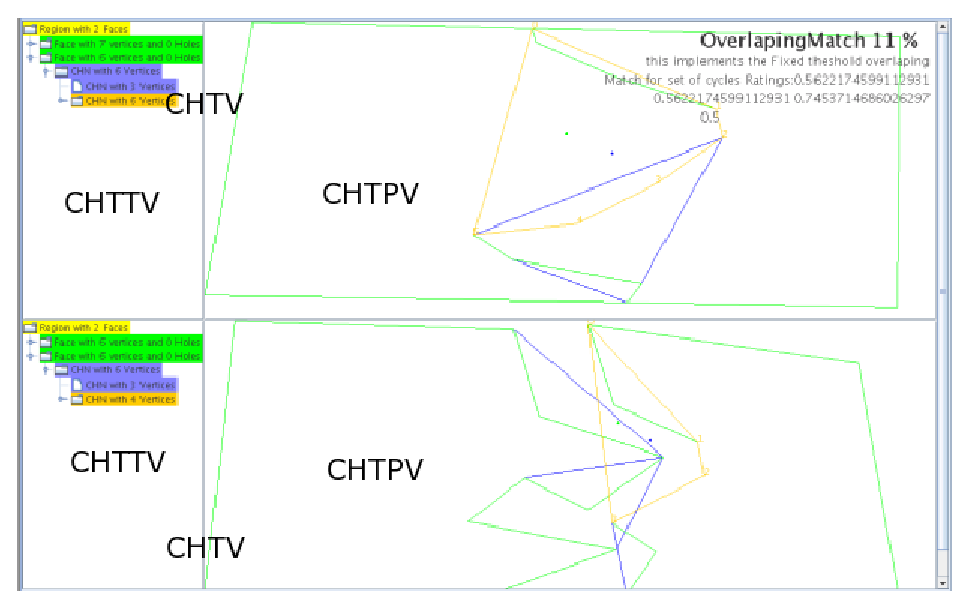
\includegraphics[scale=0.8]{MatchViewer.eps}
	\caption[MatchViewer mit allen Unteklassen] {Hier sieht man die Komponenten \textit{MatchViewer}, \textit{ConvexHullTreeViewer} (CHTV), \textit{ConvexHullTreeTreeViewer} (CHTTV) und \textit{ConvexHullPolygonViewer} (CHTPV) zusammen.\\\textit{Quelle: Eigene Darstellung}}
	\label{fig:MatchViewer}
\end{figure}

\item ConvexHullTreePolygonViewer

Diese Klasse dient dazu, einen RegionTree als Polygon darzustellen. Faces sind hier grün gefärbt, Holes rot und tieferliegende ConvexHullTreeNodes blau. Zu jedem ConvexHullTreeNode wird nicht nur der eigentliche Umfang des Polygons, sondern auch die konvexe Hülle dargestellt.

Zusätzlich beinhaltet diese Klasse ein Attribut \textit{actual}, das ein Feld von RegionTreeNodes ist. Diese Elemente werden orange dargestellt und ermöglichen das Auswählen von Elementen, falls der \textit{ConvexHullTreePolygonViewer} in einen höheren Kontext eingebunden wird.

\item ConvexHullTreeTreeViewer

Diese Klasse dient dazu einen RegionTree als Baum darzustellen. Die Darstellung dieses Baumes orientiert sich an der Darstellung, wie man sie von Verzeichnisbäumen in verschiedenen Betriebssystemen kennt.

Diese Klasse benutzt zwei Hilfsklassen:
\begin{itemize}
\item ConvexHullTreeTreeViewerNode

Diese Klasse repräsentiert ein Element des RegionTrees und kümmert sich sowohl um den rekursiven Aufbau als auch um die textuelle Beschreibung.
\item ConvexHullTreeTreeViewerRenderer

Diese Hilfsklasse kümmert sich darum, die Darstellung der einzelnen Elemente farblich zu unterscheiden. Die Farben bei der Darstellung entsprechen denen im ConvexHullTreePolygonViewer, nur dass zusätzlich noch die Farbe gelb, für das Vaterelement, die Region, benutzt wird.
\end{itemize}

Nachdem man ein Objekt dieser Klasse angelegt hat und ihm dabei den gewünschten RegionTree übergeben hat, lässt sich dieses wie jedes andere JPanel benutzen.

\item ConvexHullTreeViewer

Diese Klasse fasst die beiden Darstellungen als Baum und als Polygon zusammen. Auf der linken Seite dieser GUI-Komponente findet sich die Baum--Darstellung und auf der rechten Seite die Darstellung als Polygon. Die Verbindung zwischen den beiden wird so hergestellt, dass es möglich ist, in der Baumdarstellung ein oder mehrere Nodes zu selektieren, die dann auch in der Polygondarstellung gesondert markiert werden.

\item MatchViewer

Dieses Control zeigt einen Match an, indem zwei ConvexHullTreeViewer für die Source- und die Target-Region übereinander dargestellt werden. Die Verbindung dieser beiden wird so umgeleitet, dass die Selektion eines Elementes in einem der beiden ConvexHullTreeTreeViewer die Selektion in dem gematchten Element zur Folge hat. Konstruiert wird diese Komponente, indem man einfach ein Match übergibt. Auch diese Komponente ist von JPanel abgeleitet und lässt sich entsprechend einsetzen.

\begin{figure}
	\centering
	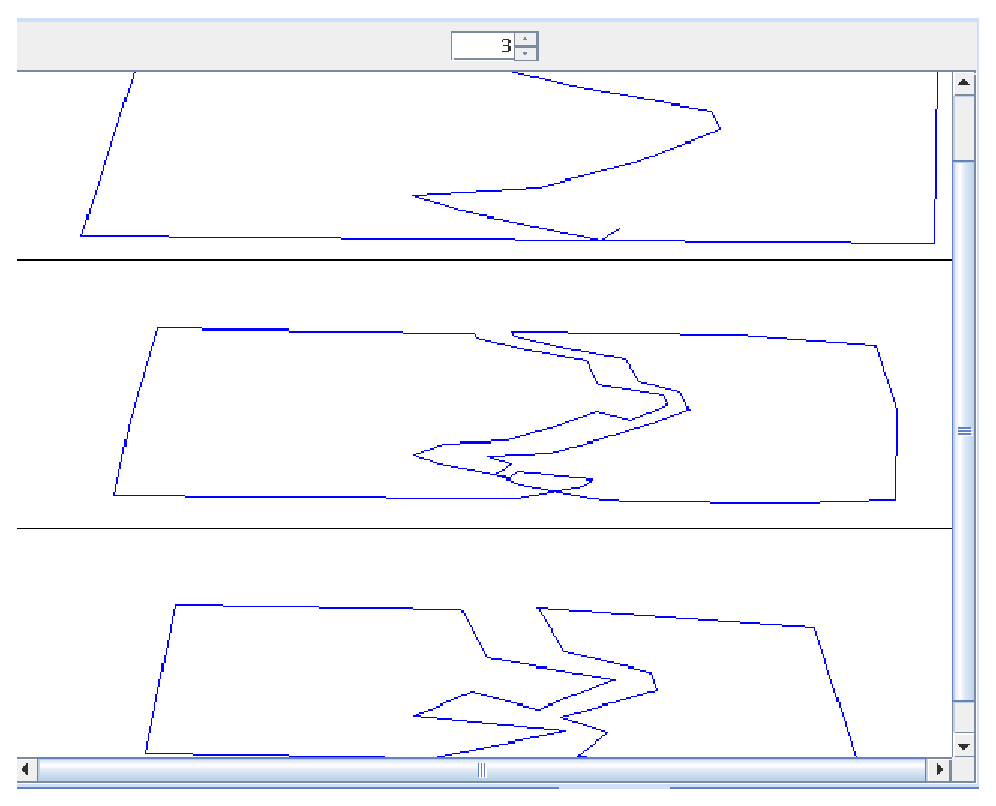
\includegraphics[scale=0.5]{Sectionviewer.eps}
	\caption[SectionViewer bestehend aus drei oneSectionViewern]{Ein \textit{SectionViewer}, bestehend aus drei \textit{oneSectionViewern}.\\\textit{Quelle: Eigene Darstellung}}
	\label{fig:SectionViewer}
\end{figure}


\item SectionViewer

Diese Klasse stellt das Ergebnis des Matchings, die erzeugten dreidimensionalen Dreiecke dar, indem eine Menge von unterschiedlichen Schnittbildern dargestellt werden. Über ein Control lässt sich die gewünschte Anzahl der Schnittbilder einstellen und dann erscheinen diese im unteren Bereich der GUI-Komponente. Die einzelnen Schnittbilder werden von der Hilfsklasse  \textbf{oneSectionViewer} gezeichnet.

Konstruiert wird der Section-Viewer, indem man diesem ein Objekt vom Typ \textit{mLine"=Rep} übergibt.


\item TriRepOutPutCanvas

Auch diese Klasse stellt ein mLineRep-Objekt dar. Allerdings erfolgt die Darstellung hier isometrisch. Die Source- und die Target-Region werden parallel zur Monitorebene dargestellt, wobei das Target nach rechtsoben verschoben wird. Die Linien des Sources sind blau, die des Targets rot. Die Linien dazwischen, also die Linien der Dreiecke, sind in grauer Farbe darghestellt.

Diese Komponente bekommt neben dem mLineRep-Objekt noch eine Ganzzahl, die den Grad der Verschiebung angibt. Diese lässt sich mittels der Methode \textbf{setTimeShift} auch nachträglich ändern. Auch wenn der Name der Klasse anderes vermuten lässt, ist diese Klasse kein Canvas, sondern ein JPanel. Der Name ist noch ein Relikt der T\o{}ssebroschen-Applikation.

\begin{figure}
	\centering
	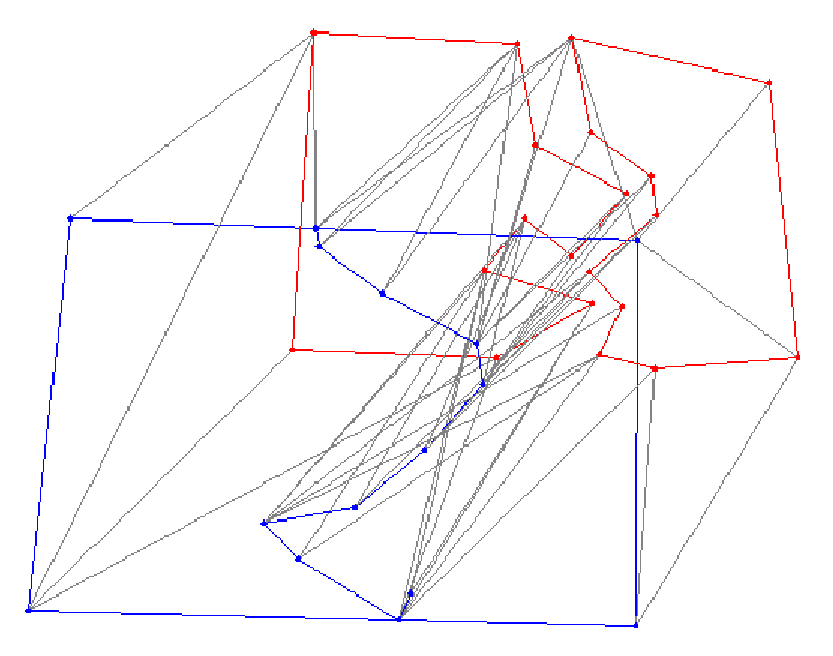
\includegraphics[scale=0.7]{TriRepOutPutCanvas.eps}
	\caption[TriRepOutputCanvas]{Ein \textit{TriRepOutputCanvas}.\\\textit{Quelle: Eigene Darstellung}}
	\label{fig:TriRepOutputCanvas}
\end{figure}




\item Tegnecanvas

Diese Klasse bildet die Zeichenfläche der Applikation. In dieser kann der Benutzer seine beiden Regionen malen. Nachdem der Benutzer dies getan hat, kann man mit den Funktionen \textbf{getFirstSnapshot} und \textbf{getSecondSnapshot} die Regionen auslesen. 

\item MCIContents

Diese Klasse vereinigt alle anderen Klassen zu der eigentlichen Applikation. Diese Klasse lässt sich entweder als Applet benutzen oder in ein JFrame einbinden, der damit eine Standalone-Applikation bildet.
\end{itemize}
\section{Die SECONDO-Algebra }\label{rialgebra}

Im Laufe der Arbeit mussten folgende Algebren verändert werden:

\subsection{PlaneSweepAlgebra}

Diese Algebra musste verwendet werden, um die Überlappung von Regionen zu berechnen. Leider konnte diese Algebra nicht im Quellcode verwendet werden, da es keine Trennung von h- und cpp-Dateien gab. Deshalb musste aus der gegebenen cpp-Datei eine Quellcode- und eine Header-Datei extrahiert werden.

\subsection{SpatialAlgebra}

Bei dem Versuch eine Region über den Quellcode zu erzeugen, gab es das Problem der nicht automatischen Mitsetzung der Bounding-Box. Außerdem fehlte eine Methode, mit deren Hilfe die Bounding-Box einer Region gesetzt werden konnte. Deshalb wurde hier die Methode \textbf{SetBoundingBox} ergänzt.

\subsection{MovingRegionAlgebra}

Es gab bislang keine Möglichkeit, \textit{RegionUnits} aus gegebenen \textit{MovingSegments} zu erzeugen. Da aber eine solche Möglichkeit  unbedingt  benötigt wird, musste ein neuer Konstruktor angelegt werden, dem man einen Vektor von \textit{MovingSegments} und ein Zeitintervall übergibt. Dieser neue Konstruktor sorgt dafür, dass die \textit{MovingSegments} in der richtigen Reihenfolge in der internen Datenstruktur abgelegt werden und dass die BoundingBox auf den richtigen Wert gesetzt wird.

Um mehrere \textit{RegionUnits} zu vereinigen, musste ein neuer Operator geschrieben werden. Dieser wird \textbf{union(uregion $u_1$,uregion $u_2$)$\rightarrow$ uregion} genannt. Dieser Operator überprüft zunächst, ob die Zeitintervalle von $u_1$ und $u_2$ gleich sind und vereinigt anschließend die beiden \textit{RegionUnits} zu einer neuen.

\subsection{RegionInterpolationAlgebra}

Dieses ist die Algebra, die speziell für diese Arbeit  angelegt wurde. Sie besteht nur aus einem einzigen Operator, der \textbf{interpolate(region  $r_1$,region $r_2$, periods $p$, real $b_1$, real $b_2$, real $b_3$,real $b_4$)$\rightarrow$ uregion} heißt. $r_1$ und $r_2$ geben die Schnappschüsse der zu erzeugenden Region"-Unit an und $p$ das zugeordnete Zeitintervall. Die optionalen Parameter $b_1,\hdots ,b_4$ geben die Gewichtungen für die Berechnung des optimales Matches an.
 %Werden diese nicht angegeben, so benutzt der Operator die in Kapitel~\vref{Kapitel4} bestimmten Werte.

